% Options for packages loaded elsewhere
\PassOptionsToPackage{unicode}{hyperref}
\PassOptionsToPackage{hyphens}{url}
%
\documentclass[
]{book}
\usepackage{lmodern}
\usepackage{amsmath}
\usepackage{ifxetex,ifluatex}
\ifnum 0\ifxetex 1\fi\ifluatex 1\fi=0 % if pdftex
  \usepackage[T1]{fontenc}
  \usepackage[utf8]{inputenc}
  \usepackage{textcomp} % provide euro and other symbols
  \usepackage{amssymb}
\else % if luatex or xetex
  \usepackage{unicode-math}
  \defaultfontfeatures{Scale=MatchLowercase}
  \defaultfontfeatures[\rmfamily]{Ligatures=TeX,Scale=1}
\fi
% Use upquote if available, for straight quotes in verbatim environments
\IfFileExists{upquote.sty}{\usepackage{upquote}}{}
\IfFileExists{microtype.sty}{% use microtype if available
  \usepackage[]{microtype}
  \UseMicrotypeSet[protrusion]{basicmath} % disable protrusion for tt fonts
}{}
\makeatletter
\@ifundefined{KOMAClassName}{% if non-KOMA class
  \IfFileExists{parskip.sty}{%
    \usepackage{parskip}
  }{% else
    \setlength{\parindent}{0pt}
    \setlength{\parskip}{6pt plus 2pt minus 1pt}}
}{% if KOMA class
  \KOMAoptions{parskip=half}}
\makeatother
\usepackage{xcolor}
\IfFileExists{xurl.sty}{\usepackage{xurl}}{} % add URL line breaks if available
\IfFileExists{bookmark.sty}{\usepackage{bookmark}}{\usepackage{hyperref}}
\hypersetup{
  pdftitle={EDV1},
  pdfauthor={Max Brede},
  hidelinks,
  pdfcreator={LaTeX via pandoc}}
\urlstyle{same} % disable monospaced font for URLs
\usepackage{color}
\usepackage{fancyvrb}
\newcommand{\VerbBar}{|}
\newcommand{\VERB}{\Verb[commandchars=\\\{\}]}
\DefineVerbatimEnvironment{Highlighting}{Verbatim}{commandchars=\\\{\}}
% Add ',fontsize=\small' for more characters per line
\usepackage{framed}
\definecolor{shadecolor}{RGB}{248,248,248}
\newenvironment{Shaded}{\begin{snugshade}}{\end{snugshade}}
\newcommand{\AlertTok}[1]{\textcolor[rgb]{0.94,0.16,0.16}{#1}}
\newcommand{\AnnotationTok}[1]{\textcolor[rgb]{0.56,0.35,0.01}{\textbf{\textit{#1}}}}
\newcommand{\AttributeTok}[1]{\textcolor[rgb]{0.77,0.63,0.00}{#1}}
\newcommand{\BaseNTok}[1]{\textcolor[rgb]{0.00,0.00,0.81}{#1}}
\newcommand{\BuiltInTok}[1]{#1}
\newcommand{\CharTok}[1]{\textcolor[rgb]{0.31,0.60,0.02}{#1}}
\newcommand{\CommentTok}[1]{\textcolor[rgb]{0.56,0.35,0.01}{\textit{#1}}}
\newcommand{\CommentVarTok}[1]{\textcolor[rgb]{0.56,0.35,0.01}{\textbf{\textit{#1}}}}
\newcommand{\ConstantTok}[1]{\textcolor[rgb]{0.00,0.00,0.00}{#1}}
\newcommand{\ControlFlowTok}[1]{\textcolor[rgb]{0.13,0.29,0.53}{\textbf{#1}}}
\newcommand{\DataTypeTok}[1]{\textcolor[rgb]{0.13,0.29,0.53}{#1}}
\newcommand{\DecValTok}[1]{\textcolor[rgb]{0.00,0.00,0.81}{#1}}
\newcommand{\DocumentationTok}[1]{\textcolor[rgb]{0.56,0.35,0.01}{\textbf{\textit{#1}}}}
\newcommand{\ErrorTok}[1]{\textcolor[rgb]{0.64,0.00,0.00}{\textbf{#1}}}
\newcommand{\ExtensionTok}[1]{#1}
\newcommand{\FloatTok}[1]{\textcolor[rgb]{0.00,0.00,0.81}{#1}}
\newcommand{\FunctionTok}[1]{\textcolor[rgb]{0.00,0.00,0.00}{#1}}
\newcommand{\ImportTok}[1]{#1}
\newcommand{\InformationTok}[1]{\textcolor[rgb]{0.56,0.35,0.01}{\textbf{\textit{#1}}}}
\newcommand{\KeywordTok}[1]{\textcolor[rgb]{0.13,0.29,0.53}{\textbf{#1}}}
\newcommand{\NormalTok}[1]{#1}
\newcommand{\OperatorTok}[1]{\textcolor[rgb]{0.81,0.36,0.00}{\textbf{#1}}}
\newcommand{\OtherTok}[1]{\textcolor[rgb]{0.56,0.35,0.01}{#1}}
\newcommand{\PreprocessorTok}[1]{\textcolor[rgb]{0.56,0.35,0.01}{\textit{#1}}}
\newcommand{\RegionMarkerTok}[1]{#1}
\newcommand{\SpecialCharTok}[1]{\textcolor[rgb]{0.00,0.00,0.00}{#1}}
\newcommand{\SpecialStringTok}[1]{\textcolor[rgb]{0.31,0.60,0.02}{#1}}
\newcommand{\StringTok}[1]{\textcolor[rgb]{0.31,0.60,0.02}{#1}}
\newcommand{\VariableTok}[1]{\textcolor[rgb]{0.00,0.00,0.00}{#1}}
\newcommand{\VerbatimStringTok}[1]{\textcolor[rgb]{0.31,0.60,0.02}{#1}}
\newcommand{\WarningTok}[1]{\textcolor[rgb]{0.56,0.35,0.01}{\textbf{\textit{#1}}}}
\usepackage{longtable,booktabs}
\usepackage{calc} % for calculating minipage widths
% Correct order of tables after \paragraph or \subparagraph
\usepackage{etoolbox}
\makeatletter
\patchcmd\longtable{\par}{\if@noskipsec\mbox{}\fi\par}{}{}
\makeatother
% Allow footnotes in longtable head/foot
\IfFileExists{footnotehyper.sty}{\usepackage{footnotehyper}}{\usepackage{footnote}}
\makesavenoteenv{longtable}
\usepackage{graphicx}
\makeatletter
\def\maxwidth{\ifdim\Gin@nat@width>\linewidth\linewidth\else\Gin@nat@width\fi}
\def\maxheight{\ifdim\Gin@nat@height>\textheight\textheight\else\Gin@nat@height\fi}
\makeatother
% Scale images if necessary, so that they will not overflow the page
% margins by default, and it is still possible to overwrite the defaults
% using explicit options in \includegraphics[width, height, ...]{}
\setkeys{Gin}{width=\maxwidth,height=\maxheight,keepaspectratio}
% Set default figure placement to htbp
\makeatletter
\def\fps@figure{htbp}
\makeatother
\setlength{\emergencystretch}{3em} % prevent overfull lines
\providecommand{\tightlist}{%
  \setlength{\itemsep}{0pt}\setlength{\parskip}{0pt}}
\setcounter{secnumdepth}{5}
\usepackage{booktabs}
\usepackage{booktabs}
\usepackage{longtable}
\usepackage{array}
\usepackage{multirow}
\usepackage{wrapfig}
\usepackage{float}
\usepackage{colortbl}
\usepackage{pdflscape}
\usepackage{tabu}
\usepackage{threeparttable}
\usepackage{threeparttablex}
\usepackage[normalem]{ulem}
\usepackage{makecell}
\usepackage{xcolor}
\ifluatex
  \usepackage{selnolig}  % disable illegal ligatures
\fi
\usepackage[]{natbib}
\bibliographystyle{apalike}

\title{EDV1}
\author{Max Brede}
\date{2021-01-02}

\begin{document}
\maketitle

{
\setcounter{tocdepth}{1}
\tableofcontents
}
\hypertarget{vorwort}{%
\chapter{Vorwort}\label{vorwort}}

Dieses mit \texttt{bookdown} erstellte Dokument ist das über das Wintersemester 2020 hinweg wachsende Skript zur Übung ``PSY\_B\_11-2: Computerunterstützte Datenanalyse I'' der CAU zu Kiel.

\hypertarget{lehrplan}{%
\chapter{Lehrplan}\label{lehrplan}}

\hypertarget{semesterplan}{%
\section{Semesterplan}\label{semesterplan}}

\hypertarget{uxfcbungsformat}{%
\section{Übungsformat}\label{uxfcbungsformat}}

Die Übung soll zur Hälfte in 45-minütigen Sitzungen im Vorlesungsformat zur Vorstellung der Funktionen und zur anderen Hälfte als 45-minütige praktische Übung stattfinden.
Es wird pro Übungs-Sitzung ein Übungszettel ausgegeben, der mit Hilfe der in der Zugehörigen Vorlesung besprochenen Funktionen bearbeitet werden können soll.
Diese Zettel sollen nach der jeweiligen Vorlesung für die Übungen vorbereitet werden, in denen der Zettel dann besprochen und mögliche Fragen geklärt werden.
Nach den Übungssitzungen haben die Studierenden dann eine Woche Zeit, zusätzliche Hausaufgaben zu bearbeiten.

Eine Ausnahme von diesem Ablauf ist die erste Sitzung, in der organisatorisches und Grundlagen in 90 minütigem Vorlesungsstil besprochen werden sollen. Auch nach dieser Sitzung werden aber Übungszettel und Hausaufgaben ausgegeben.

\hypertarget{lehrziele-fuxfcr-jede-sitzung}{%
\section{Lehrziele für jede Sitzung}\label{lehrziele-fuxfcr-jede-sitzung}}

Die Studierenden können nach dem Absolvieren der Übung\ldots{}

\hypertarget{einheit-1}{%
\subsubsection*{Einheit 1}\label{einheit-1}}
\addcontentsline{toc}{subsubsection}{Einheit 1}

\begin{itemize}
\tightlist
\item
  Vor- und Nachteile von R und RStudio nennen und diese installieren.
\item
  erklären was Funktionen und was Argumente sind.
\item
  die Hilfe benutzen.
\item
  das Environment von R benutzen um Objekte anzulegen und zu löschen.
\end{itemize}

\hypertarget{einheit-2}{%
\subsubsection*{Einheit 2}\label{einheit-2}}
\addcontentsline{toc}{subsubsection}{Einheit 2}

\begin{itemize}
\tightlist
\item
  Vektoren erstellen, tranformieren und indizieren.
\item
  verschiedene Datenformate in R erstellen, benutzen und in einander überführen.
\end{itemize}

\hypertarget{einheit-3}{%
\subsubsection*{Einheit 3}\label{einheit-3}}
\addcontentsline{toc}{subsubsection}{Einheit 3}

\begin{itemize}
\tightlist
\item
  Pakete installieren und benutzen.
\item
  mit Hilfe des ``\texttt{tidyverse}'' Datensätze erstellen, ergänzen, sortieren und indizieren.
\end{itemize}

\hypertarget{einheit-4}{%
\subsubsection*{Einheit 4}\label{einheit-4}}
\addcontentsline{toc}{subsubsection}{Einheit 4}

\begin{itemize}
\tightlist
\item
  Faktoren erstellen.
\item
  Daten auf Gruppenebene aggregieren.
\item
  Häufigkeiten auszählen und tabellarisch darstellen.
\end{itemize}

\hypertarget{einheit-5}{%
\subsubsection*{Einheit 5}\label{einheit-5}}
\addcontentsline{toc}{subsubsection}{Einheit 5}

\begin{itemize}
\tightlist
\item
  Daten auf Gruppenebene noch besser aggregieren.
\item
  Datensätze aus verschiedenen Formaten einlesen.
\end{itemize}

\hypertarget{einheit-6}{%
\subsubsection*{Einheit 6}\label{einheit-6}}
\addcontentsline{toc}{subsubsection}{Einheit 6}

\begin{itemize}
\tightlist
\item
  Datensätze kombinieren und pivotieren.
\item
  eine Anzahl von Grafiken erstellen.
\end{itemize}

\hypertarget{einheit-7}{%
\subsubsection*{Einheit 7}\label{einheit-7}}
\addcontentsline{toc}{subsubsection}{Einheit 7}

\begin{itemize}
\tightlist
\item
  kompliziertere Grafiken erstellen.
\end{itemize}

\hypertarget{einheit-8}{%
\subsubsection*{Einheit 8}\label{einheit-8}}
\addcontentsline{toc}{subsubsection}{Einheit 8}

\begin{itemize}
\tightlist
\item
  die Funktionsschreibweise lesen und anwenden.
\item
  erfolgreich an der Klausur teilnehmen.
\end{itemize}

\hypertarget{pruxfcfungsleistung}{%
\section{Prüfungsleistung}\label{pruxfcfungsleistung}}

Die Studierenden \textbf{müssen} während des Semesters die nach den Übungssitzungen ausgegebenen Hausaufgaben innerhalb einer Woche sinnvoll bearbeitet abgeben.

Mit maximal einer nicht sinnvoll bearbeiteten Serie werden die Studierenden zur Klausur am Ende des Semesters zugelassen.

\hypertarget{vorlesung-i---rste-schritte}{%
\chapter{Vorlesung I - Rste Schritte}\label{vorlesung-i---rste-schritte}}

\hypertarget{organisatorisches}{%
\section{Organisatorisches}\label{organisatorisches}}

\hypertarget{semesterplan-1}{%
\subsection*{Semesterplan}\label{semesterplan-1}}
\addcontentsline{toc}{subsection}{Semesterplan}

\begin{table}[H]
\centering\begingroup\fontsize{15}{17}\selectfont

\begin{tabular}{l|l|l|l}
\hline
Einheit & Vorlesung & Übungswoche & Thema\\
\hline
1 & 2.11.20 & keine Übung & Grundlagen und Begriffe\\
\hline
2 & 16.11.20 & KW 48 & Vektoren und Indizierung\\
\hline
 &  &  & Datenformate erstellen und transformieren\\
\hline
3 & 30.11.20 & KW 50 & Pakete installieren und benutzen\\
\hline
 &  &  & Datensätze erstellen und ergänzen können\\
\hline
 &  &  & Datensätze sortieren und indizieren können\\
\hline
4 & 14.12.20 & KW 1 & Faktoren\\
\hline
 &  &  & deskriptive Kennwerte\\
\hline
 &  &  & Aggregation I\\
\hline
5 & 11.01.21 & KW 3 & Aggregation II\\
\hline
 &  &  & In- und Export von Datensätzen\\
\hline
6 & 25.01.21 & KW 5 & Grafische Darstellungen I\\
\hline
7 & 08.02.21 & KW 7 & Grafische Darstellungen II\\
\hline
8 & 22.02.21 & keine Übung & Puffer\\
\hline
 &  &  & Probeklausur\\
\hline
\end{tabular}
\endgroup{}
\end{table}

\hypertarget{uxfcbungsablauf}{%
\subsection*{Übungsablauf}\label{uxfcbungsablauf}}
\addcontentsline{toc}{subsection}{Übungsablauf}

Die Übung wird zur Hälfte als Vorlesung, zur anderen Hälfte in Kleingruppen abgehalten.

Die Daten sind im Kalender und im Semesterplan im Olat ersichtlich.

\hypertarget{pruxfcfungsleistung-1}{%
\subsection*{Prüfungsleistung}\label{pruxfcfungsleistung-1}}
\addcontentsline{toc}{subsection}{Prüfungsleistung}

Die Prüfungsleistung in dieser Veranstaltung besteht aus:

\begin{enumerate}
\def\labelenumi{\arabic{enumi}.}
\tightlist
\item
  Dem \emph{regelmäßigen Bearbeiten} und \emph{Bestehen} von Hausaufgaben. Diese werden über das OLAT ausgeteilt und abgegeben, zu jeder Veranstaltung wird eine neue Serie herausgegeben. Das Bestehen der Hausaufgaben ist nötig, um zur Klausur zugelassen zu werden.

  \begin{itemize}
  \tightlist
  \item
    Als \emph{Bestanden} gilt eine Serie, wenn alle Aufgaben \textbf{sinnvoll} bearbeitet wurden.
  \item
    Unter \emph{regelmäßigem Bearbeiten} versteht sich das Bestehen aller Serien \textbf{mit einer Ausnahme}. \medskip  
  \end{itemize}
\item
  Im Klausurzeitraum findet an einem Tag eine praktische Prüfung statt.
\end{enumerate}

\hypertarget{einfuxfchrung}{%
\section{Einführung}\label{einfuxfchrung}}

\hypertarget{rste-schritte}{%
\subsection*{Rste Schritte}\label{rste-schritte}}
\addcontentsline{toc}{subsection}{Rste Schritte}

Diese Veranstaltung und das zugehörige Material sollen Ihnen einen Einstieg in das computergestützte Aufbereiten und Auswerten von empirischen Daten bieten.
Dazu werden wir auf die von ihren Autoren als `software environment for statistical computing and graphics' bezeichnete, freie Umgebung R zurückgreifen.

\hypertarget{wozu-brauche-ich-das}{%
\subsection*{Wozu brauche ich das?}\label{wozu-brauche-ich-das}}
\addcontentsline{toc}{subsection}{Wozu brauche ich das?}

\begin{center}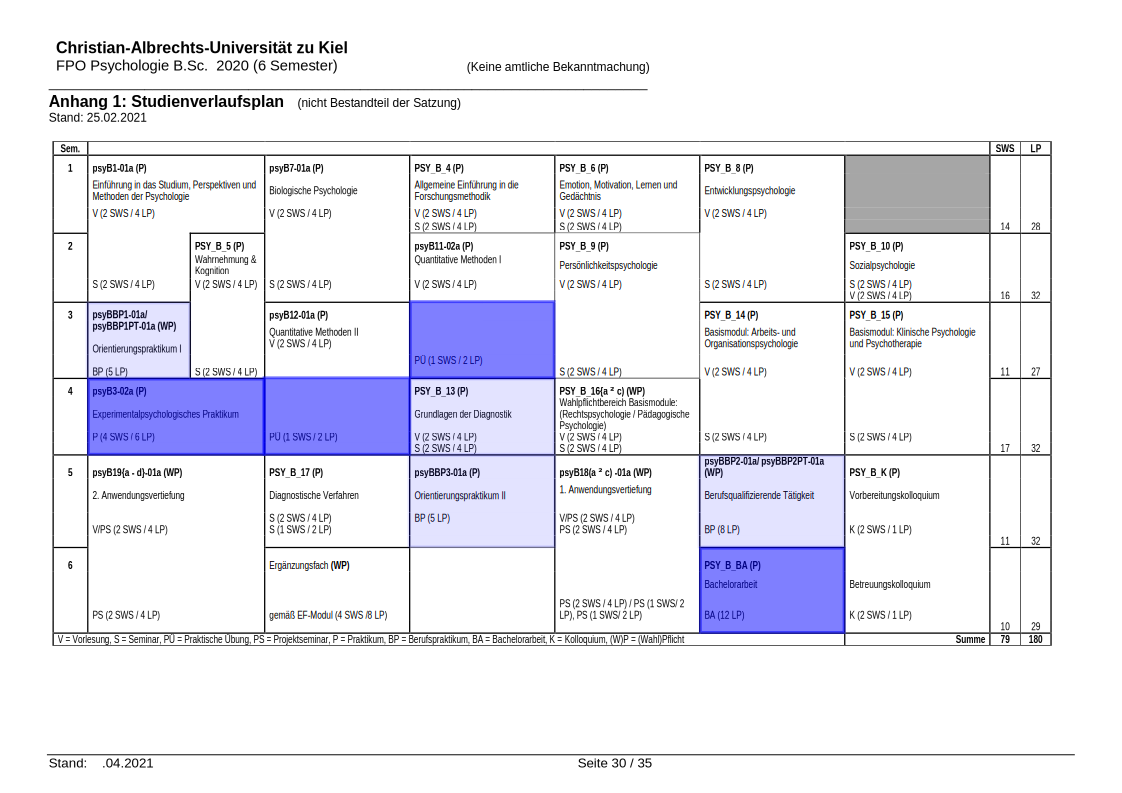
\includegraphics[width=0.8\linewidth]{imgs/relevanz} \end{center}

\hypertarget{warum-r}{%
\subsection*{Warum R ?}\label{warum-r}}
\addcontentsline{toc}{subsection}{Warum R ?}

\hypertarget{und-nicht-spss}{%
\subsubsection*{(\ldots und nicht SPSS\ldots)}\label{und-nicht-spss}}
\addcontentsline{toc}{subsubsection}{(\ldots und nicht SPSS\ldots)}

\begin{table}[H]
\centering
\begin{tabular}[t]{l|l|l}
\hline
  & SPSS & R\\
\hline
 &  & \\
\hline
Pro & einfache Bedienung & das `CRAN` (Comprehensive R Archive Network)\\
\hline
 & weit verbreitet & kostenlos\\
\hline
 &  & macht was angewiesen ist\\
\hline
 &  & \\
\hline
Contra & kann nicht alles & etwas Gewöhnung notwendig\\
\hline
 & relativ kostenintensive Lizenzen & \\
\hline
 & nimmt vieles ab & \\
\hline
 & nicht beliebig erweiterbar & \\
\hline
\end{tabular}
\end{table}

Aber die viel wichtigeren Argumente:
R kann \textbf{Alles}

\begin{center}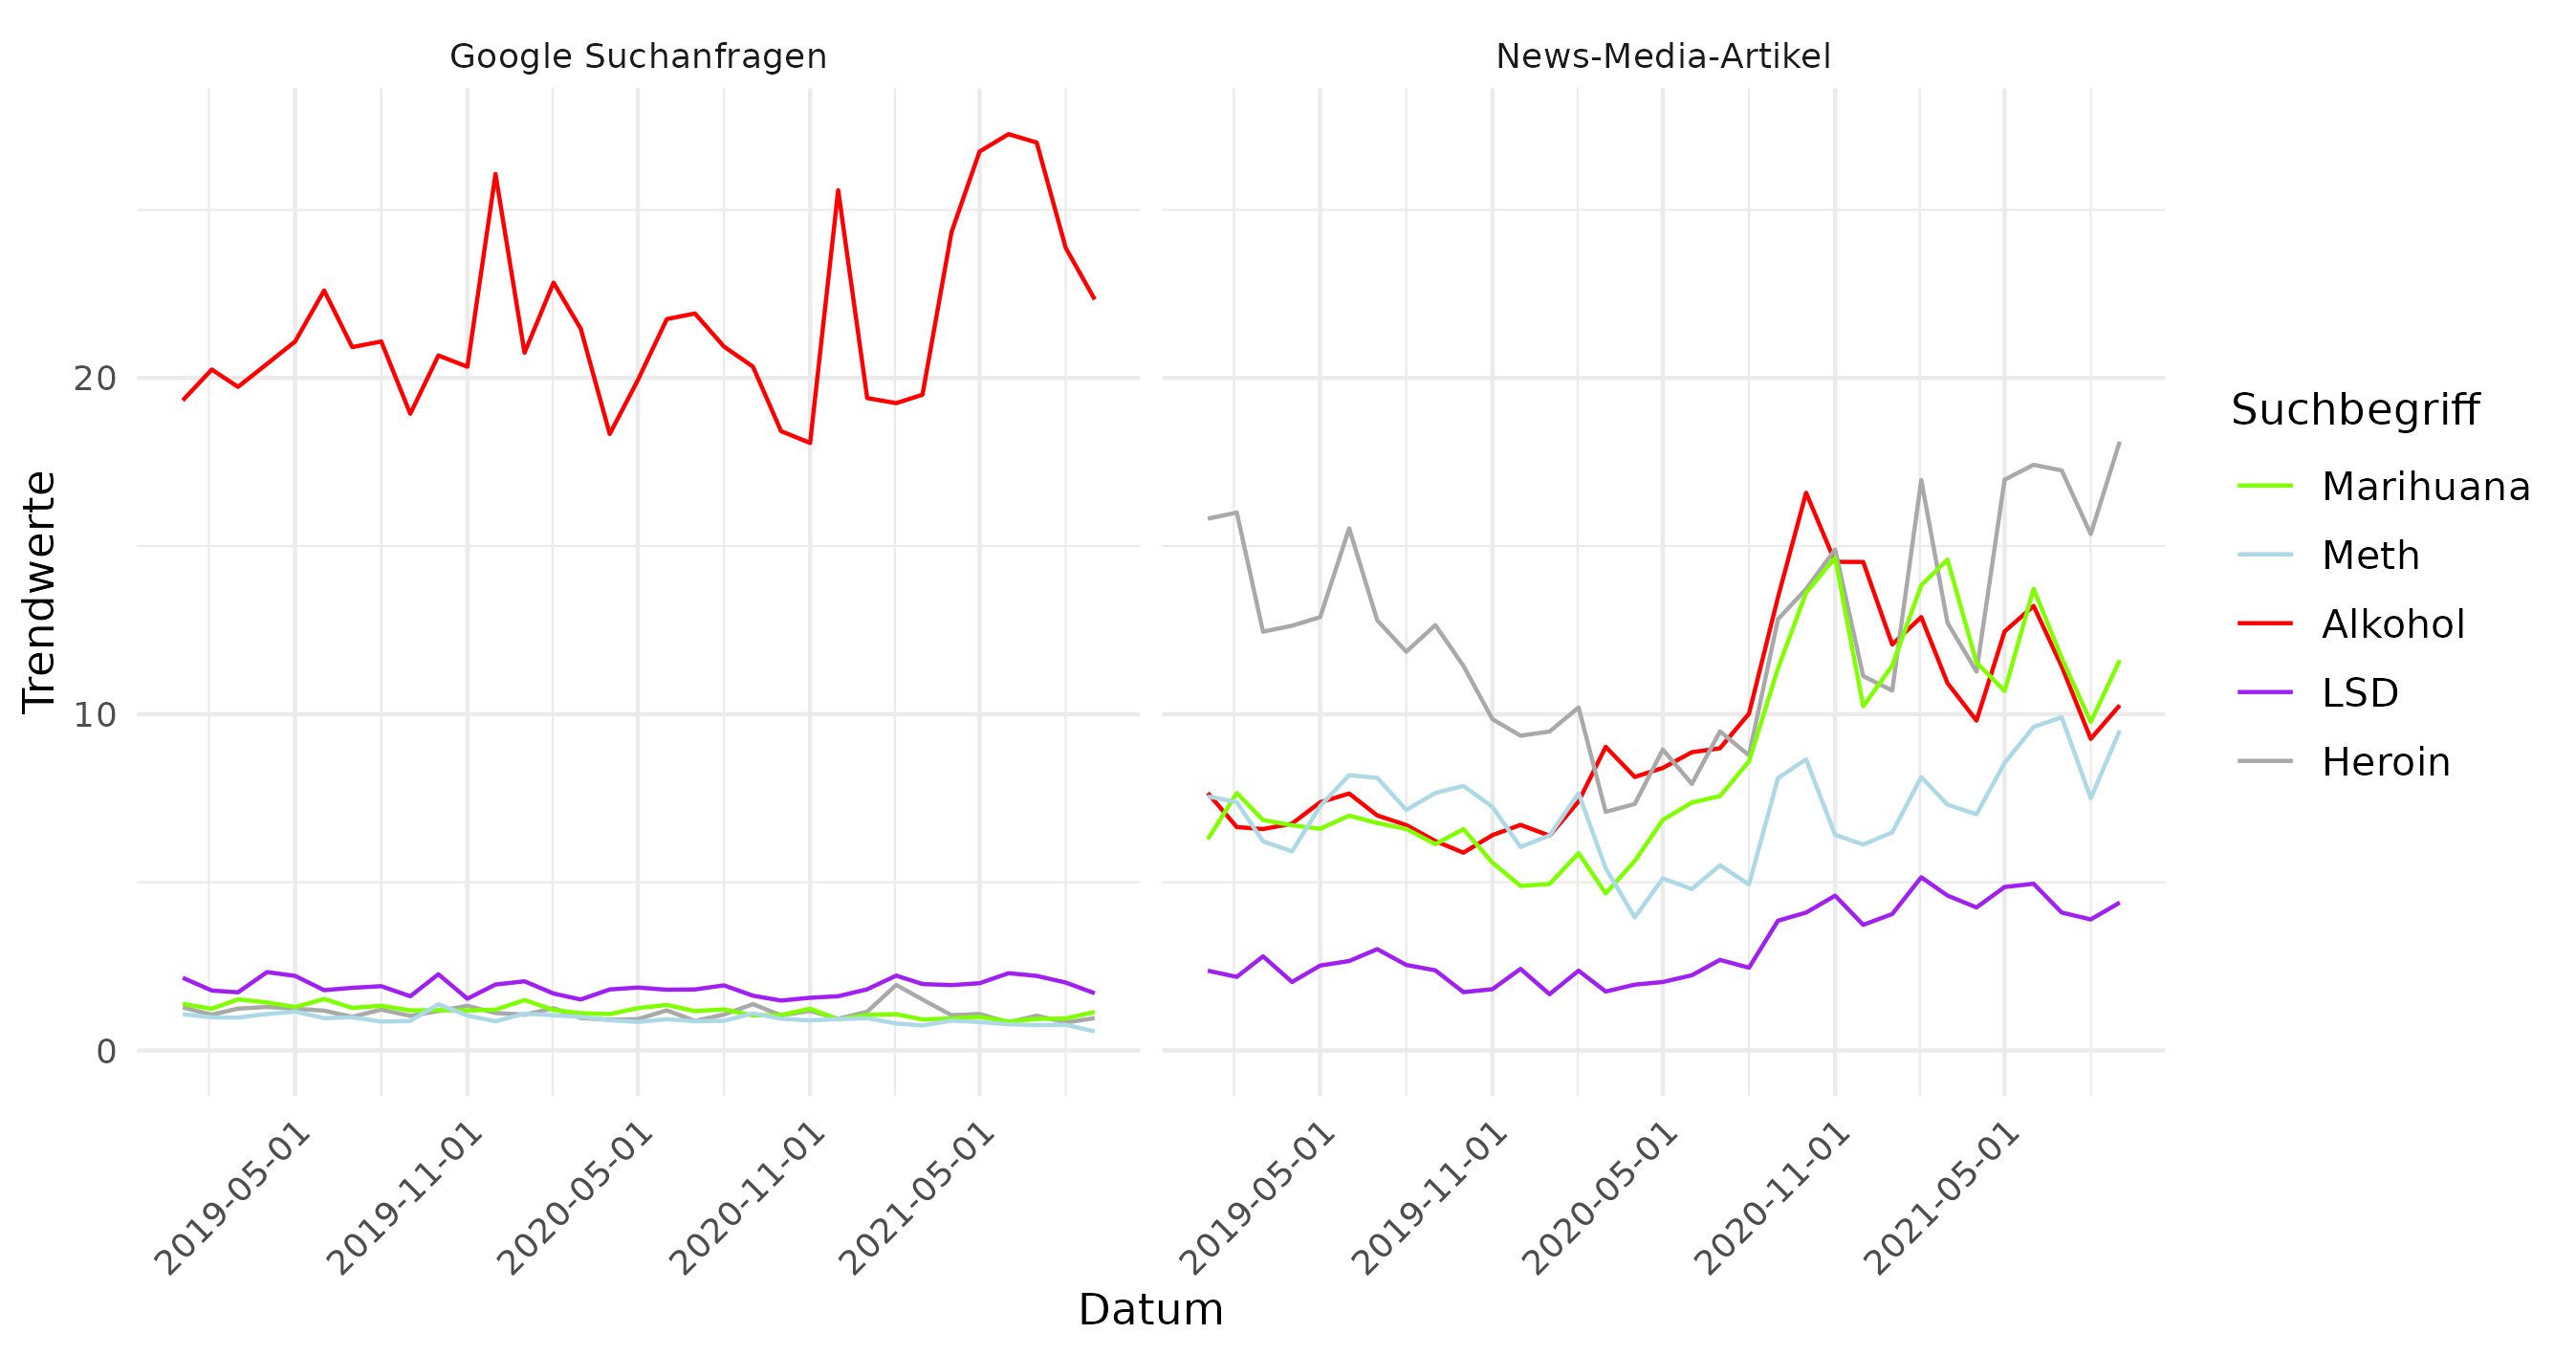
\includegraphics[width=0.7\linewidth]{imgs/drugs} \end{center}

R macht \textbf{Spass}

\begin{center}\includegraphics[width=0.45\linewidth]{imgs/thumbnail} \end{center}

\hypertarget{literatur}{%
\subsection*{Literatur}\label{literatur}}
\addcontentsline{toc}{subsection}{Literatur}

Die Veranstaltung orientiert sich an:

\begin{enumerate}
\def\labelenumi{\arabic{enumi}.}
\item
  \citet{wollschlaegerKompaktSchnelleEinstieg2016} . R kompakt.(Link aus dem Uni-Netz).
\item
  \citet{grolemundDataScience} . R for Data Science (Link).
\end{enumerate}

\hypertarget{installation-verwendung}{%
\subsection*{Installation \& Verwendung}\label{installation-verwendung}}
\addcontentsline{toc}{subsection}{Installation \& Verwendung}

Es wird die Verwendung der grafischen Benutzeroberfläche \href{http://www.rstudio.com}{RStudio} empfohlen.

Beachten Sie, dass für die Verwendung von RStudio zuvor eine Basisinstallation von \href{http://cran.r-project.org}{R} erfolgen muss:

\begin{enumerate}
\def\labelenumi{\arabic{enumi}.}
\item
  (R) herunterladen und installieren.
\item
  (RStudio) herunterladen und installieren.
\end{enumerate}

\hypertarget{benutzeroberfluxe4che-rstudio}{%
\subsection*{Benutzeroberfläche RStudio}\label{benutzeroberfluxe4che-rstudio}}
\addcontentsline{toc}{subsection}{Benutzeroberfläche RStudio}

\begin{figure}
\centering
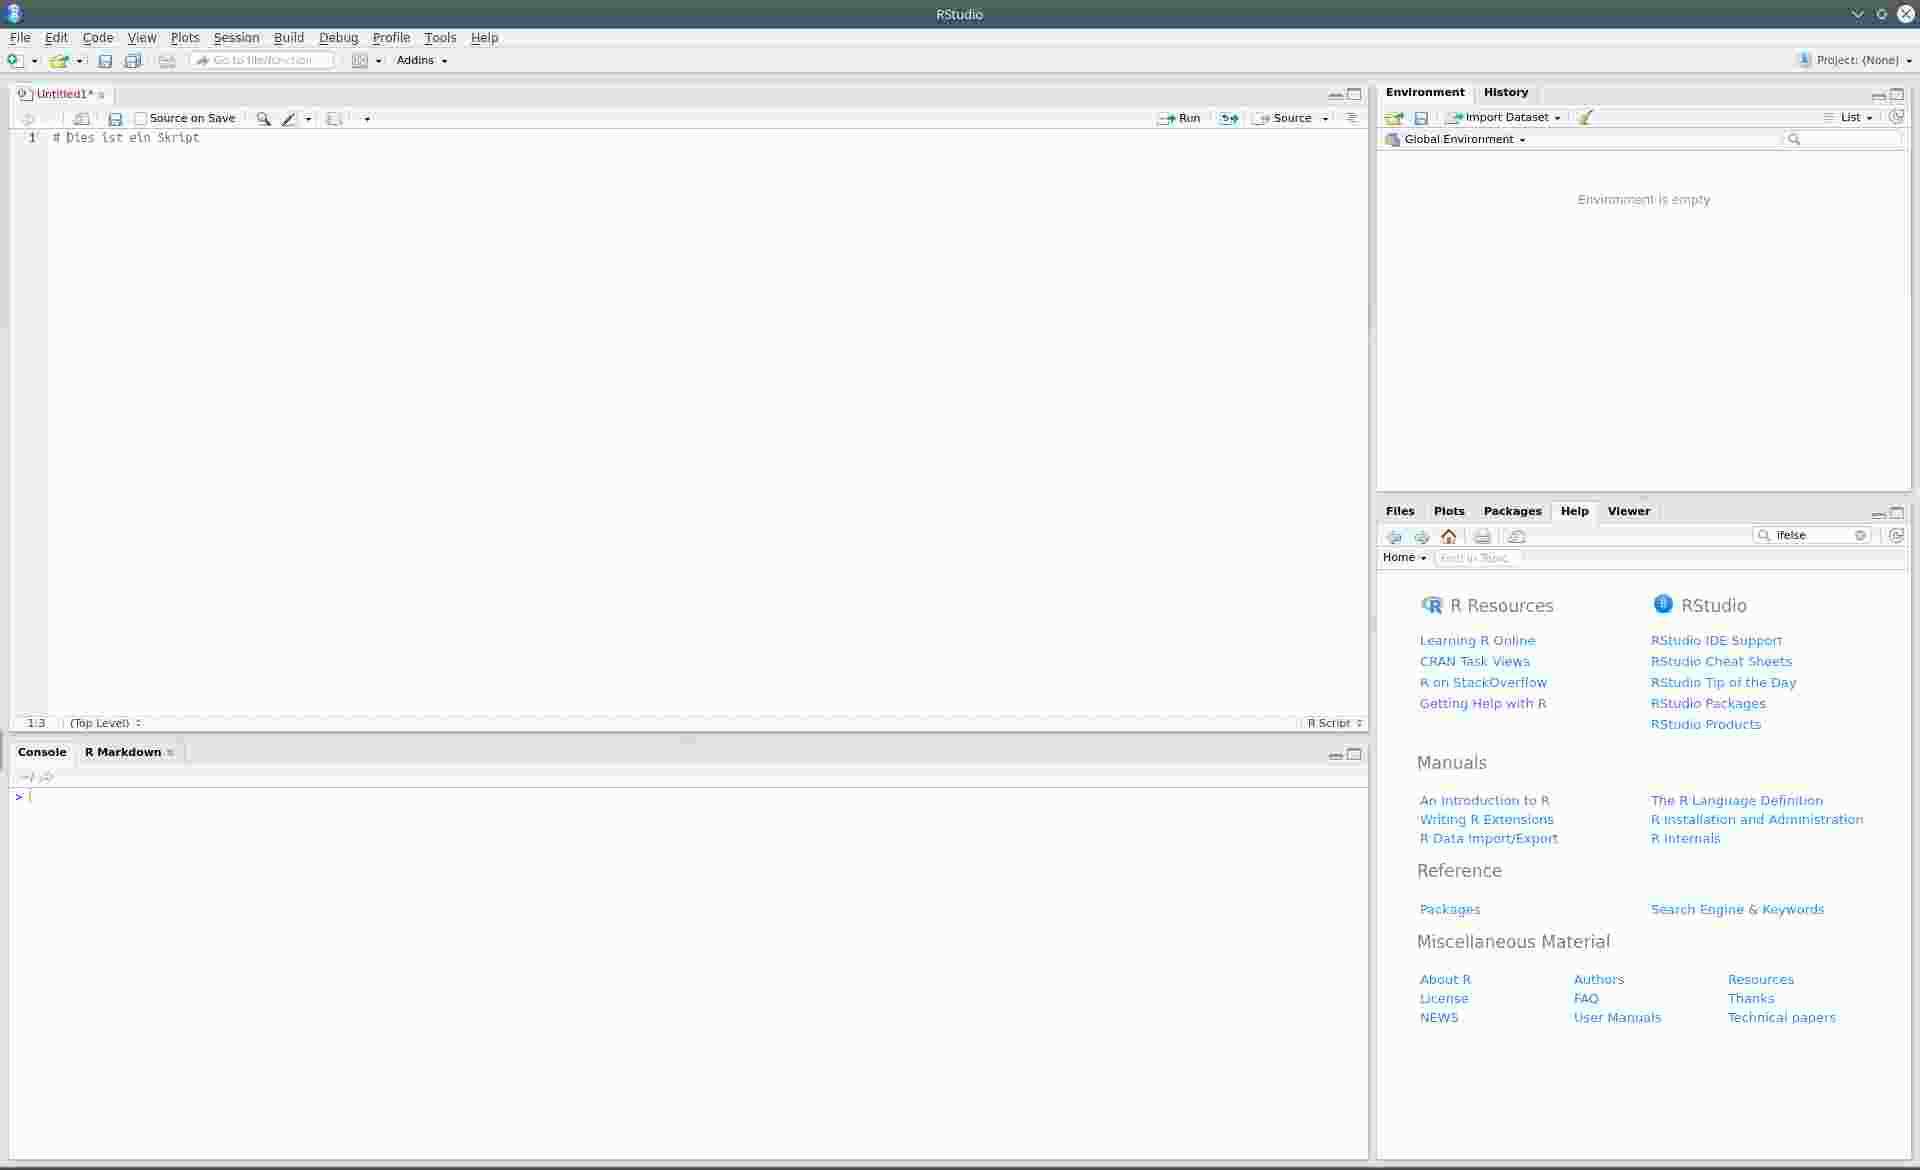
\includegraphics[width=0.6\textwidth,height=\textheight]{imgs/RStudio_003.jpg}
\caption{Benutzeroberfläche von RStudio. Oben links: Editor; unten links: Konsole; oben rechts: Environment bzw. History; unten rechts: Files, Plots, Help, etc.}
\end{figure}

\hypertarget{allgemeine-hinweise}{%
\subsection*{Allgemeine Hinweise}\label{allgemeine-hinweise}}
\addcontentsline{toc}{subsection}{Allgemeine Hinweise}

\begin{itemize}
\tightlist
\item
  Verwenden Sie die Konsole (unten links) nur für einzeilige Berechnungen beim ``Ausprobieren''
\item
  Verwenden Sie stets den Editor (oben links), um mehrzeilige Berechnungen direkt in ein Skript zu schreiben
\item
  Kommentieren Sie Ihren Code ausreichend und sinnvoll mit Hilfe des \texttt{\#}-Zeichens
\item
  Speichern Sie Ihr Skript unter einem sinnvollen Namen in einem sinnvoll benannten Verzeichnis ab
\end{itemize}

\begin{itemize}
\tightlist
\item
  Speichern Sie regelmäßig mit Strg+S zwischen
\item
  Eine einzelne Skript-Zeile (diejenige, in der sich der Cursor befindet) oder zuvor markierter Code lassen sich mit Strg+Enter ausführen
\item
  In der Konsole bricht ESC die Eingabe ab
\end{itemize}

\hypertarget{zum-besseren-verstuxe4ndnis}{%
\subsection*{Zum besseren Verständnis}\label{zum-besseren-verstuxe4ndnis}}
\addcontentsline{toc}{subsection}{Zum besseren Verständnis}

In diesem Skript enthalten die grau hinterlegten Zeilen R-Input, die weiß hinterlegten Zeilen den R-Output. Ein ganz einfaches Beispiel zum Ausprobieren: Die simple Berechnung von 1 + 1.

\begin{Shaded}
\begin{Highlighting}[]
\DecValTok{1} \SpecialCharTok{+} \DecValTok{1}
\end{Highlighting}
\end{Shaded}

\begin{verbatim}
## [1] 2
\end{verbatim}

\hypertarget{ausdruxfccke-in-der-r-konsole}{%
\subsection*{Ausdrücke in der R-Konsole}\label{ausdruxfccke-in-der-r-konsole}}
\addcontentsline{toc}{subsection}{Ausdrücke in der R-Konsole}

Anweisungen in R funktionieren grundsätzlich über das Ausführen von Ausdrücken. Dabei werden Ausdrücke entweder durch Semikolons oder Zeilenumbrüche beendet.

\begin{Shaded}
\begin{Highlighting}[]
\DecValTok{1} \SpecialCharTok{+} \DecValTok{1}\NormalTok{; }\DecValTok{2} \SpecialCharTok{+} \DecValTok{2}\NormalTok{;}
\end{Highlighting}
\end{Shaded}

\begin{verbatim}
## [1] 2
\end{verbatim}

\begin{verbatim}
## [1] 4
\end{verbatim}

\begin{Shaded}
\begin{Highlighting}[]
\DecValTok{1}\SpecialCharTok{+}\DecValTok{1}
\end{Highlighting}
\end{Shaded}

\begin{verbatim}
## [1] 2
\end{verbatim}

\begin{Shaded}
\begin{Highlighting}[]
\DecValTok{2}\SpecialCharTok{+}\DecValTok{2}
\end{Highlighting}
\end{Shaded}

\begin{verbatim}
## [1] 4
\end{verbatim}

\hypertarget{kommentare}{%
\subsection*{Kommentare}\label{kommentare}}
\addcontentsline{toc}{subsection}{Kommentare}

R bietet außerdem die Möglichkeit, im Code Anmerkungen zu machen, die beim Ausführen ignoriert werden. Diese werden mit einem \texttt{\#}-Symbol eingeleitet.

\begin{Shaded}
\begin{Highlighting}[]
\DecValTok{1} \SpecialCharTok{+} \DecValTok{1} \DocumentationTok{\#\#\# +1 +1}
\end{Highlighting}
\end{Shaded}

\begin{verbatim}
## [1] 2
\end{verbatim}

\begin{Shaded}
\begin{Highlighting}[]
\CommentTok{\#Dies ist ein Kommentar}
\end{Highlighting}
\end{Shaded}

Nutzen Sie Kommentare innerhalb Ihrer Skripte, um Arbeitsschritte kenntlich zu machen und zu erklären. Die übersichtliche Gestaltung Ihrer Skripte ist von wirklich großem Vorteil bei der Arbeit mit R. Dies kann nicht oft genug betont werden.

\hypertarget{grundlegende-rechenoperationen}{%
\section{Grundlegende Rechenoperationen}\label{grundlegende-rechenoperationen}}

\hypertarget{addition-subtraktion}{%
\subsection*{Addition, Subtraktion}\label{addition-subtraktion}}
\addcontentsline{toc}{subsection}{Addition, Subtraktion}

\begin{Shaded}
\begin{Highlighting}[]
\DecValTok{2} \SpecialCharTok{+} \DecValTok{3}  
\end{Highlighting}
\end{Shaded}

\begin{verbatim}
## [1] 5
\end{verbatim}

\begin{Shaded}
\begin{Highlighting}[]
\DecValTok{28} \SpecialCharTok{{-}} \DecValTok{5}  
\end{Highlighting}
\end{Shaded}

\begin{verbatim}
## [1] 23
\end{verbatim}

\hypertarget{multiplikation-division}{%
\subsection*{Multiplikation, Division}\label{multiplikation-division}}
\addcontentsline{toc}{subsection}{Multiplikation, Division}

\begin{Shaded}
\begin{Highlighting}[]
\DecValTok{2} \SpecialCharTok{*} \DecValTok{21}   
\end{Highlighting}
\end{Shaded}

\begin{verbatim}
## [1] 42
\end{verbatim}

\begin{Shaded}
\begin{Highlighting}[]
\DecValTok{92} \SpecialCharTok{/} \DecValTok{4}
\end{Highlighting}
\end{Shaded}

\begin{verbatim}
## [1] 23
\end{verbatim}

\hypertarget{rechenregeln}{%
\subsection*{Rechenregeln}\label{rechenregeln}}
\addcontentsline{toc}{subsection}{Rechenregeln}

\begin{Shaded}
\begin{Highlighting}[]
\DecValTok{1}\SpecialCharTok{+}\DecValTok{1}\SpecialCharTok{*}\DecValTok{1}\SpecialCharTok{+}\DecValTok{1}\SpecialCharTok{*}\NormalTok{(}\DecValTok{1}\SpecialCharTok{+}\DecValTok{1}\NormalTok{)}\SpecialCharTok{+}\DecValTok{1}
\end{Highlighting}
\end{Shaded}

\begin{verbatim}
## [1] 5
\end{verbatim}

Wie man sieht, befolgt R die Punkt-vor-Strich-Regel und berücksichtigt Klammerung.

\hypertarget{potenz-quadratwurzel-squareroot-betrag-absolute}{%
\subsection*{Potenz, Quadratwurzel (``squareroot''), Betrag (``absolute'')}\label{potenz-quadratwurzel-squareroot-betrag-absolute}}
\addcontentsline{toc}{subsection}{Potenz, Quadratwurzel (``squareroot''), Betrag (``absolute'')}

\begin{Shaded}
\begin{Highlighting}[]
\DecValTok{3}\SpecialCharTok{\^{}}\DecValTok{2}
\end{Highlighting}
\end{Shaded}

\begin{verbatim}
## [1] 9
\end{verbatim}

\begin{Shaded}
\begin{Highlighting}[]
\FunctionTok{sqrt}\NormalTok{(}\DecValTok{9}\NormalTok{)}
\end{Highlighting}
\end{Shaded}

\begin{verbatim}
## [1] 3
\end{verbatim}

\begin{Shaded}
\begin{Highlighting}[]
\FunctionTok{abs}\NormalTok{(}\SpecialCharTok{{-}}\DecValTok{42}\NormalTok{)}
\end{Highlighting}
\end{Shaded}

\begin{verbatim}
## [1] 42
\end{verbatim}

\hypertarget{runden}{%
\subsection*{Runden}\label{runden}}
\addcontentsline{toc}{subsection}{Runden}

\begin{Shaded}
\begin{Highlighting}[]
\NormalTok{pi}
\end{Highlighting}
\end{Shaded}

\begin{verbatim}
## [1] 3.141593
\end{verbatim}

\begin{Shaded}
\begin{Highlighting}[]
\FunctionTok{round}\NormalTok{(pi)}
\end{Highlighting}
\end{Shaded}

\begin{verbatim}
## [1] 3
\end{verbatim}

\begin{Shaded}
\begin{Highlighting}[]
\FunctionTok{round}\NormalTok{(pi, }\AttributeTok{digits=}\DecValTok{2}\NormalTok{)}
\end{Highlighting}
\end{Shaded}

\begin{verbatim}
## [1] 3.14
\end{verbatim}

\begin{Shaded}
\begin{Highlighting}[]
\FunctionTok{round}\NormalTok{(pi, }\AttributeTok{digits=}\DecValTok{3}\NormalTok{)}
\end{Highlighting}
\end{Shaded}

\begin{verbatim}
## [1] 3.142
\end{verbatim}

\hypertarget{aufgabe}{%
\subsection*{Aufgabe}\label{aufgabe}}
\addcontentsline{toc}{subsection}{Aufgabe}

\begin{Shaded}
\begin{Highlighting}[]
\FunctionTok{round}\NormalTok{(pi, }\AttributeTok{digits =} \DecValTok{0}\NormalTok{) }\SpecialCharTok{*} \DecValTok{3} \DocumentationTok{\#\#\# + 5}
\end{Highlighting}
\end{Shaded}

\hypertarget{was-kommt-raus}{%
\subsubsection*{Was kommt raus?}\label{was-kommt-raus}}
\addcontentsline{toc}{subsubsection}{Was kommt raus?}

\begin{enumerate}
\def\labelenumi{\Alph{enumi})}
\tightlist
\item
  \texttt{pi}
\item
  \texttt{14}
\item
  eine Fehlermeldung
\item
  \texttt{9}
\item
  \texttt{NULL}
\end{enumerate}

\hypertarget{ausdruxfccke-funktionen-argumente}{%
\section{Ausdrücke, Funktionen, Argumente}\label{ausdruxfccke-funktionen-argumente}}

\hypertarget{funktionen-argumente}{%
\subsection*{Funktionen \& Argumente}\label{funktionen-argumente}}
\addcontentsline{toc}{subsection}{Funktionen \& Argumente}

In R werden sehr häufig \emph{Funktionen} verwendet. Diese repräsentieren eine Reihe von Anweisungen, die beim Aufrufen mit spezifischen Parametern ausgeführt werden sollen. Diese Parameter werde in Form von \emph{Argumenten} übergeben.
Beispielsweise enthält die Funktion \texttt{round()} die nötigen Anweisungen, um eine Zahl zu runden. Hierfür erwartet \texttt{round()} die zu rundende Zahl und die Anzahl an Nachkommastellen auf die zu runden ist.
Man schreibt immer \emph{Funktionsname}(\emph{Argumentliste}). Bei Funktionen müssen \emph{immer} runde Klammern vorhanden sein, auch wenn keine einzelnen Argumente vorgegeben werden.

Es gibt \emph{obligatorische Argumente}, ohne deren Übergabe das Aufrufen einer Funktion zu einer Fehlermeldung führt:
\scriptsize

\begin{Shaded}
\begin{Highlighting}[]
\FunctionTok{round}\NormalTok{(pi)}
\end{Highlighting}
\end{Shaded}

\begin{verbatim}
## [1] 3
\end{verbatim}

\begin{Shaded}
\begin{Highlighting}[]
\FunctionTok{round}\NormalTok{() }\DocumentationTok{\#\#\# Funktionsaufruf ohne Argument}
\end{Highlighting}
\end{Shaded}

\begin{verbatim}
## Error in eval(expr, envir, enclos): 0 arguments passed to 'round' which requires 1 or 2 arguments
\end{verbatim}

\ldots{} und \emph{optionale Argumente}:
\scriptsize

\begin{Shaded}
\begin{Highlighting}[]
\FunctionTok{round}\NormalTok{(pi, }\AttributeTok{digits=}\DecValTok{3}\NormalTok{)}
\end{Highlighting}
\end{Shaded}

\begin{verbatim}
## [1] 3.142
\end{verbatim}

\begin{Shaded}
\begin{Highlighting}[]
\FunctionTok{round}\NormalTok{(pi, }\AttributeTok{digits=}\NormalTok{pi)}
\end{Highlighting}
\end{Shaded}

\begin{verbatim}
## [1] 3.142
\end{verbatim}

\begin{Shaded}
\begin{Highlighting}[]
\FunctionTok{round}\NormalTok{(pi, }\AttributeTok{digits=}\DecValTok{15}\NormalTok{)}
\end{Highlighting}
\end{Shaded}

\begin{verbatim}
## [1] 3.141593
\end{verbatim}

Gibt man den Namen eines Arguments nicht an, entscheidet die Position in der Liste über die Interpretation des Arguments durch R. \textbf{Achtung: Fehlerquelle!}
\scriptsize

\begin{Shaded}
\begin{Highlighting}[]
\FunctionTok{round}\NormalTok{(}\DecValTok{1}\SpecialCharTok{/}\DecValTok{42}\NormalTok{, }\DecValTok{3}\NormalTok{)}
\end{Highlighting}
\end{Shaded}

\begin{verbatim}
## [1] 0.024
\end{verbatim}

\begin{Shaded}
\begin{Highlighting}[]
\FunctionTok{round}\NormalTok{(}\DecValTok{3}\NormalTok{, }\DecValTok{1}\SpecialCharTok{/}\DecValTok{42}\NormalTok{)}
\end{Highlighting}
\end{Shaded}

\begin{verbatim}
## [1] 3
\end{verbatim}

\hypertarget{objekte}{%
\section{Objekte}\label{objekte}}

\emph{Objekte} sind für den späteren Gebrauch mit einem Namen versehene und im Arbeitsspeicher abgelegte Ergebnisse von Ausdrücken.
Dabei ist Objekt der Überbegriff für eine Vielzahl von möglichen Datenstrukturen.

Ein paar Beispiele für Datenstrukturen in R:

\begin{itemize}
\tightlist
\item
  eindimensionale Vektoren (vector)
\item
  mehrdimensionale Matrizen (matrix)
\item
  Funktionen(function)
\end{itemize}

\hypertarget{objekte-benennen}{%
\subsection*{Objekte benennen}\label{objekte-benennen}}
\addcontentsline{toc}{subsection}{Objekte benennen}

Wählen Sie kurze, aber aussagekräftige Objektnamen! Objektnamen dürfen dabei enthalten: Buchstaben, Zahlen, Punkte, Unterstriche

\textbf{Achtung:}

\begin{itemize}
\tightlist
\item
  Immer mit einem Buchstaben beginnen
\item
  Groß-/Kleinschreibung ist relevant
\item
  Keine anderen Sonderzeichen
\item
  Keine durch R reservierte Namen von Funktionen, Konstanten, etc. (z.B. ``mean'', ``pi'', ``if'', etc.) (im Zweifel Überprüfen mit \texttt{exists()})
\end{itemize}

Hier nochmal der nachdrückliche Hinweis: Tun Sie sich selbst den Gefallen, Ihre Objekte eindeutig und nachvollziehbar zu benennen!

\hypertarget{zuweisungen-an-objekte}{%
\subsection*{Zuweisungen an Objekte}\label{zuweisungen-an-objekte}}
\addcontentsline{toc}{subsection}{Zuweisungen an Objekte}

Ergebnisse von Ausdrücken können benannten Objekten zugewiesen werden.

Dabei sind folgende Ausdrücke äquivalent:

\begin{Shaded}
\begin{Highlighting}[]
\NormalTok{firstObject }\OtherTok{=} \DecValTok{42}
\DecValTok{42} \OtherTok{{-}\textgreater{}}\NormalTok{ firstObject}
\NormalTok{firstObject }\OtherTok{\textless{}{-}} \DecValTok{42}
\end{Highlighting}
\end{Shaded}

Die letzte Möglichkeit stellt dabei die Beste im Hinblick auf Übersichtlichkeit und Eindeutigkeit dar.

\hypertarget{verwenden-von-objekten}{%
\subsection*{Verwenden von Objekten:}\label{verwenden-von-objekten}}
\addcontentsline{toc}{subsection}{Verwenden von Objekten:}

Die Objektnamen können dann synonym zu ihrem Inhalt verwendet werden.

\begin{Shaded}
\begin{Highlighting}[]
\NormalTok{firstObject }\SpecialCharTok{+} \DecValTok{1}\NormalTok{; }\DecValTok{42} \SpecialCharTok{+} \DecValTok{1}\NormalTok{;}
\end{Highlighting}
\end{Shaded}

\begin{verbatim}
## [1] 43
\end{verbatim}

\begin{verbatim}
## [1] 43
\end{verbatim}

\hypertarget{objekte-ausgeben}{%
\subsection*{Objekte ausgeben}\label{objekte-ausgeben}}
\addcontentsline{toc}{subsection}{Objekte ausgeben}

Um diese Ausgabe nachzuholen gibt es folgende Möglichkeiten:

\begin{Shaded}
\begin{Highlighting}[]
\FunctionTok{print}\NormalTok{(firstObject)}
\end{Highlighting}
\end{Shaded}

\begin{verbatim}
## [1] 42
\end{verbatim}

\begin{Shaded}
\begin{Highlighting}[]
\NormalTok{firstObject}
\end{Highlighting}
\end{Shaded}

\begin{verbatim}
## [1] 42
\end{verbatim}

Diese beiden Versionen sind faktisch dieselbe, da das einfache Aufrufen eines Variablennamens implizit als ein Aufruf von \texttt{print()} interpretiert wird.

\begin{Shaded}
\begin{Highlighting}[]
\NormalTok{(object2 }\OtherTok{\textless{}{-}}\NormalTok{ firstObject}\SpecialCharTok{\^{}}\DecValTok{2}\NormalTok{)}
\end{Highlighting}
\end{Shaded}

\begin{verbatim}
## [1] 1764
\end{verbatim}

Bei Setzen eines Befehls in Klammern wird die durch ihn ausgelöste Änderung ausgegeben, im Beispiel die Zuweisung des Ergebnisses zum neuen Objekt \texttt{object2}.

Diese Methode ist eine gute Variante, Zwischenergebnisse regelmäßig zu kontrollieren.

\hypertarget{objekte-anzeigen-lassen}{%
\subsection*{Objekte anzeigen lassen}\label{objekte-anzeigen-lassen}}
\addcontentsline{toc}{subsection}{Objekte anzeigen lassen}

Alle Objekte im Workspace anzeigen lassen:

\begin{Shaded}
\begin{Highlighting}[]
\FunctionTok{ls}\NormalTok{()}
\end{Highlighting}
\end{Shaded}

\begin{verbatim}
## [1] "a"           "firstObject" "object2"    
## [4] "plan"
\end{verbatim}

Diese Operation braucht man später nicht unbedingt, da alle angelegten Objekte auch im Environment-Tab in RStudio einsehen kann. Am Anfang kann diese Funktion aber helfen, sich über die Abläufe klar zu werden.

\begin{figure}
\centering
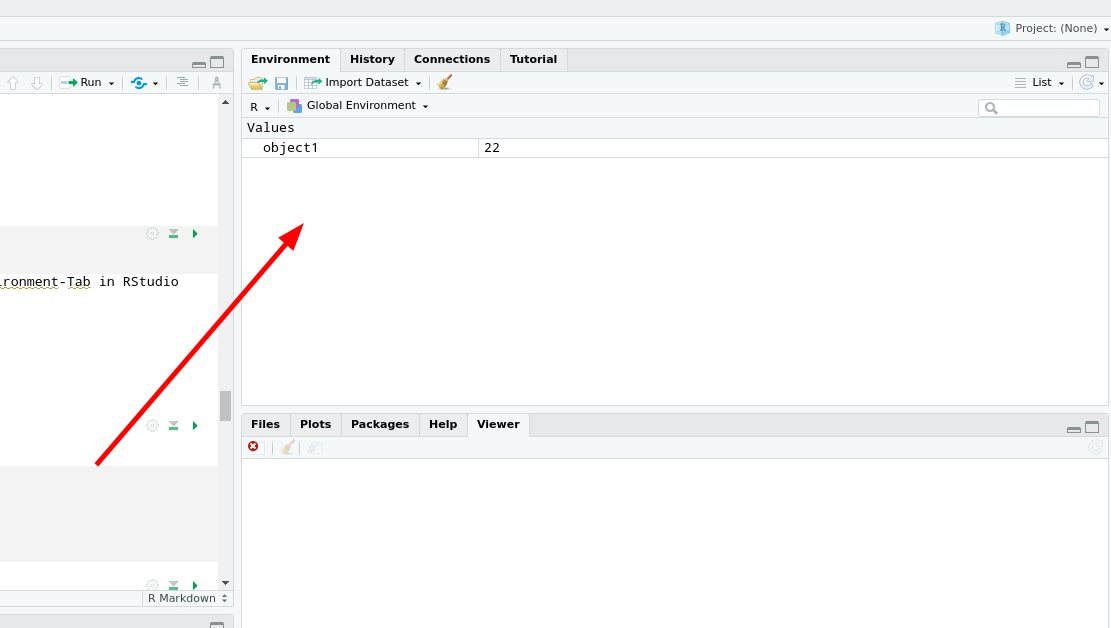
\includegraphics[width=0.4\textwidth,height=\textheight]{imgs/environment.png}
\caption{Environment}
\end{figure}

\hypertarget{objekte-entfernen}{%
\subsection*{Objekte entfernen}\label{objekte-entfernen}}
\addcontentsline{toc}{subsection}{Objekte entfernen}

Vorhandene Objekte lassen sich dann wie folgt entfernen:

\begin{Shaded}
\begin{Highlighting}[]
\FunctionTok{ls}\NormalTok{()}
\end{Highlighting}
\end{Shaded}

\begin{verbatim}
## [1] "a"           "firstObject" "object2"    
## [4] "plan"
\end{verbatim}

\begin{Shaded}
\begin{Highlighting}[]
\FunctionTok{rm}\NormalTok{(object2)}
\FunctionTok{ls}\NormalTok{()}
\end{Highlighting}
\end{Shaded}

\begin{verbatim}
## [1] "a"           "firstObject" "plan"
\end{verbatim}

Mit \texttt{rm(list=ls())} lassen sich alle Objekte aus dem Workspace entfernen.

\begin{Shaded}
\begin{Highlighting}[]
\FunctionTok{ls}\NormalTok{()}
\end{Highlighting}
\end{Shaded}

\begin{verbatim}
## [1] "a"           "firstObject" "plan"
\end{verbatim}

\begin{Shaded}
\begin{Highlighting}[]
\FunctionTok{rm}\NormalTok{(}\AttributeTok{list=}\FunctionTok{ls}\NormalTok{())}
\FunctionTok{ls}\NormalTok{()}
\end{Highlighting}
\end{Shaded}

\begin{verbatim}
## character(0)
\end{verbatim}

\hypertarget{datentypen}{%
\subsection*{Datentypen}\label{datentypen}}
\addcontentsline{toc}{subsection}{Datentypen}

\small

In R, wie in so gut wie jeder anderen Sprache, werden Objekte in unterschiedliche Subtypen gegliedert, die sich auf die in ihnen gespeicherten Informationen beziehen:

\begin{tabular}[t]{l|l|l}
\hline
Beschreibung & Beispiel & Datentyp\\
\hline
leere Menge & `NULL` & `NULL`\\
\hline
logische Werte & `TRUE, FALSE, T,  F` & `logical`\\
\hline
ganze und reelle Zahlen & `42` & `numeric`\\
\hline
Buchstaben- o. Zeichenfolgen (immer in <br> Anführungszeichen) & `beware of the leopard.` & `character`\\
\hline
\end{tabular}

Dabei ist das hier keine vollständige Liste, für den Anfang reicht sie aber.

\texttt{mode()} gibt den Datentyp des übergebenen Arguments aus (braucht man selten, hier nur für das Beispiel):

\begin{Shaded}
\begin{Highlighting}[]
\FunctionTok{mode}\NormalTok{(answer)}
\end{Highlighting}
\end{Shaded}

\begin{verbatim}
## [1] "numeric"
\end{verbatim}

\begin{Shaded}
\begin{Highlighting}[]
\FunctionTok{mode}\NormalTok{(}\StringTok{\textquotesingle{}answer\textquotesingle{}}\NormalTok{)}
\end{Highlighting}
\end{Shaded}

\begin{verbatim}
## [1] "character"
\end{verbatim}

\hypertarget{datentypen-konvertieren}{%
\subsection*{Datentypen konvertieren}\label{datentypen-konvertieren}}
\addcontentsline{toc}{subsection}{Datentypen konvertieren}

\scriptsize

\texttt{as.character(answer)} konvertiert den Datentyp des Objekts von \texttt{numeric} nach \texttt{character} ohne den ursprünglichen Eintrag von \texttt{answer} zu überschreiben.

\begin{Shaded}
\begin{Highlighting}[]
\FunctionTok{mode}\NormalTok{(answer)}
\end{Highlighting}
\end{Shaded}

\begin{verbatim}
## [1] "numeric"
\end{verbatim}

\begin{Shaded}
\begin{Highlighting}[]
\FunctionTok{as.character}\NormalTok{(answer)}
\end{Highlighting}
\end{Shaded}

\begin{verbatim}
## [1] "42"
\end{verbatim}

\begin{Shaded}
\begin{Highlighting}[]
\FunctionTok{mode}\NormalTok{(answer)}
\end{Highlighting}
\end{Shaded}

\begin{verbatim}
## [1] "numeric"
\end{verbatim}

Um das zu erreichen muss das Objekt überschrieben werden:

\begin{Shaded}
\begin{Highlighting}[]
\NormalTok{answer }\OtherTok{\textless{}{-}} \FunctionTok{as.character}\NormalTok{(answer)}
\FunctionTok{mode}\NormalTok{(answer)}
\end{Highlighting}
\end{Shaded}

\begin{verbatim}
## [1] "character"
\end{verbatim}

Mit \texttt{answer} als character-Element lässt sich nicht mehr rechnen:

\begin{Shaded}
\begin{Highlighting}[]
\NormalTok{answer }\SpecialCharTok{*} \DecValTok{2}
\end{Highlighting}
\end{Shaded}

\begin{verbatim}
## Error in answer * 2: non-numeric argument to binary operator
\end{verbatim}

Um das dann wieder zu ermöglichen muss das Objekt zurück nach numeric konvertiert werden:

\begin{Shaded}
\begin{Highlighting}[]
\NormalTok{answer }\OtherTok{\textless{}{-}} \FunctionTok{as.numeric}\NormalTok{(answer)}
\FunctionTok{mode}\NormalTok{(answer)}
\end{Highlighting}
\end{Shaded}

\begin{verbatim}
## [1] "numeric"
\end{verbatim}

\begin{Shaded}
\begin{Highlighting}[]
\NormalTok{answer }\SpecialCharTok{*} \DecValTok{2}
\end{Highlighting}
\end{Shaded}

\begin{verbatim}
## [1] 84
\end{verbatim}

Weitere Beispiele für Konvertierung:

\begin{Shaded}
\begin{Highlighting}[]
\FunctionTok{as.numeric}\NormalTok{(}\StringTok{"42"}\NormalTok{) }\DocumentationTok{\#\#\# konvertiert character nach numeric}
\end{Highlighting}
\end{Shaded}

\begin{verbatim}
## [1] 42
\end{verbatim}

\begin{Shaded}
\begin{Highlighting}[]
\FunctionTok{as.numeric}\NormalTok{(}\ConstantTok{TRUE}\NormalTok{) }\DocumentationTok{\#\#\# konvertiert logical nach numeric}
\end{Highlighting}
\end{Shaded}

\begin{verbatim}
## [1] 1
\end{verbatim}

\begin{Shaded}
\begin{Highlighting}[]
\FunctionTok{as.logical}\NormalTok{(}\DecValTok{0}\NormalTok{)  }\DocumentationTok{\#\#\# konvertiert numeric nach logical}
\end{Highlighting}
\end{Shaded}

\begin{verbatim}
## [1] FALSE
\end{verbatim}

\begin{Shaded}
\begin{Highlighting}[]
\FunctionTok{as.logical}\NormalTok{(}\DecValTok{1}\NormalTok{)  }\DocumentationTok{\#\#\# konvertiert numeric nach logical }
\end{Highlighting}
\end{Shaded}

\begin{verbatim}
## [1] TRUE
\end{verbatim}

\begin{Shaded}
\begin{Highlighting}[]
\FunctionTok{as.logical}\NormalTok{(}\DecValTok{23}\NormalTok{)  }\DocumentationTok{\#\#\# konvertiert numeric nach logical}
\end{Highlighting}
\end{Shaded}

\begin{verbatim}
## [1] TRUE
\end{verbatim}

\begin{Shaded}
\begin{Highlighting}[]
\FunctionTok{as.logical}\NormalTok{(}\StringTok{"true"}\NormalTok{)  }\DocumentationTok{\#\#\# konvertiert character nach logical}
\end{Highlighting}
\end{Shaded}

\begin{verbatim}
## [1] TRUE
\end{verbatim}

\hypertarget{logische-werte-operatoren-und-verknuxfcpfungen}{%
\subsection*{Logische Werte, Operatoren und Verknüpfungen}\label{logische-werte-operatoren-und-verknuxfcpfungen}}
\addcontentsline{toc}{subsection}{Logische Werte, Operatoren und Verknüpfungen}

Logische Vergleiche, Verknüpfungen und andere Operatoren:

\begin{table}[H]
\centering\begingroup\fontsize{15}{17}\selectfont

\begin{tabular}[t]{l|l}
\hline
Operator & Operation\\
\hline
`==` & ist gleich\\
\hline
`!=` & ist ungleich\\
\hline
> & ist größer\\
\hline
>= & ist größer gleich\\
\hline
< & ist kleiner\\
\hline
<= & ist kleiner gleich\\
\hline
`!` & logisches NICHT\\
\hline
\& & logisches UND\\
\hline
`|` & logisches ODER\\
\hline
`isTRUE()` & gibt an, ob übergebenes Argument TRUE ist\\
\hline
 & \\
\hline
\end{tabular}
\endgroup{}
\end{table}

Das Ergebnis eines logischen Vergleichs sind logische Werte:\\
WAHR: \texttt{TRUE\ =\ T\ =\ 1}\\
FALSCH: \texttt{FALSE\ =\ F\ =\ 0}

Beispiele:

\begin{Shaded}
\begin{Highlighting}[]
\DecValTok{1} \SpecialCharTok{==} \DecValTok{2}
\end{Highlighting}
\end{Shaded}

\begin{verbatim}
## [1] FALSE
\end{verbatim}

\begin{Shaded}
\begin{Highlighting}[]
\DecValTok{1} \SpecialCharTok{!=} \DecValTok{2}
\end{Highlighting}
\end{Shaded}

\begin{verbatim}
## [1] TRUE
\end{verbatim}

\begin{Shaded}
\begin{Highlighting}[]
\DecValTok{1} \SpecialCharTok{\textless{}} \DecValTok{2}
\end{Highlighting}
\end{Shaded}

\begin{verbatim}
## [1] TRUE
\end{verbatim}

\begin{Shaded}
\begin{Highlighting}[]
\DecValTok{1} \SpecialCharTok{\textgreater{}=} \DecValTok{2}
\end{Highlighting}
\end{Shaded}

\begin{verbatim}
## [1] FALSE
\end{verbatim}

\begin{Shaded}
\begin{Highlighting}[]
\DecValTok{1}\SpecialCharTok{\textgreater{}}\DecValTok{2} \SpecialCharTok{\&} \DecValTok{1}\SpecialCharTok{\textless{}=}\DecValTok{3}
\end{Highlighting}
\end{Shaded}

\begin{verbatim}
## [1] FALSE
\end{verbatim}

\begin{Shaded}
\begin{Highlighting}[]
\DecValTok{2}\SpecialCharTok{\textgreater{}}\DecValTok{1} \SpecialCharTok{|} \DecValTok{1}\SpecialCharTok{!=}\DecValTok{1}
\end{Highlighting}
\end{Shaded}

\begin{verbatim}
## [1] TRUE
\end{verbatim}

\begin{Shaded}
\begin{Highlighting}[]
\DecValTok{6}\SpecialCharTok{\textgreater{}}\DecValTok{5} \SpecialCharTok{\&} \SpecialCharTok{!}\NormalTok{(}\DecValTok{2}\SpecialCharTok{\textless{}=}\DecValTok{1}\NormalTok{)}
\end{Highlighting}
\end{Shaded}

\begin{verbatim}
## [1] TRUE
\end{verbatim}

\begin{Shaded}
\begin{Highlighting}[]
\FunctionTok{isTRUE}\NormalTok{(}\DecValTok{1} \SpecialCharTok{==} \DecValTok{1}\NormalTok{)}
\end{Highlighting}
\end{Shaded}

\begin{verbatim}
## [1] TRUE
\end{verbatim}

\begin{Shaded}
\begin{Highlighting}[]
\NormalTok{(}\DecValTok{1} \SpecialCharTok{==} \DecValTok{1}\NormalTok{)}
\end{Highlighting}
\end{Shaded}

\begin{verbatim}
## [1] TRUE
\end{verbatim}

\hypertarget{aufgabe-1}{%
\subsection*{Aufgabe}\label{aufgabe-1}}
\addcontentsline{toc}{subsection}{Aufgabe}

\hypertarget{was-kommt-raus-1}{%
\subsubsection*{Was kommt raus?}\label{was-kommt-raus-1}}
\addcontentsline{toc}{subsubsection}{Was kommt raus?}

\begin{Shaded}
\begin{Highlighting}[]
\NormalTok{(}\DecValTok{2} \SpecialCharTok{\textgreater{}} \DecValTok{1} \SpecialCharTok{\&} \DecValTok{1} \SpecialCharTok{\textless{}} \DecValTok{3}\NormalTok{) }\SpecialCharTok{|} \DecValTok{1} \SpecialCharTok{!=} \DecValTok{1}
\end{Highlighting}
\end{Shaded}

\begin{enumerate}
\def\labelenumi{\Alph{enumi})}
\tightlist
\item
  \texttt{TRUE}
\item
  \texttt{FALSE}
\item
  \texttt{NULL}
\end{enumerate}

\hypertarget{umgang-mit-dezimalzahlen}{%
\subsection*{Umgang mit Dezimalzahlen:}\label{umgang-mit-dezimalzahlen}}
\addcontentsline{toc}{subsection}{Umgang mit Dezimalzahlen:}

\hypertarget{was-kommt-hier-raus}{%
\subsubsection*{Was kommt hier raus?}\label{was-kommt-hier-raus}}
\addcontentsline{toc}{subsubsection}{Was kommt hier raus?}

\begin{Shaded}
\begin{Highlighting}[]
\FloatTok{0.1} \SpecialCharTok{+} \FloatTok{0.2} \SpecialCharTok{==} \FloatTok{0.3}
\end{Highlighting}
\end{Shaded}

\begin{enumerate}
\def\labelenumi{\Alph{enumi})}
\tightlist
\item
  \texttt{TRUE}
\item
  \texttt{FALSE}
\item
  \texttt{NULL}
\end{enumerate}

\begin{Shaded}
\begin{Highlighting}[]
\FloatTok{0.1} \SpecialCharTok{+} \FloatTok{0.2} \SpecialCharTok{==} \FloatTok{0.3}
\end{Highlighting}
\end{Shaded}

\begin{verbatim}
## [1] FALSE
\end{verbatim}

\textbf{0.1 + 0.2 != 0.3?}

`Falsches' Ergebnis ist Resultat von Repräsentation von Gleitkommazahlen im Speicher des Rechners.\\
Die Funktion \texttt{all.equal()} löst dieses Problem.

\begin{Shaded}
\begin{Highlighting}[]
\FunctionTok{all.equal}\NormalTok{(}\AttributeTok{target=}\FloatTok{0.1+0.2}\NormalTok{, }\AttributeTok{current=}\FloatTok{0.3}\NormalTok{)}
\end{Highlighting}
\end{Shaded}

\begin{verbatim}
## [1] TRUE
\end{verbatim}

Mit dem \texttt{tolerance}-Argument lässt sich der Bereich der akzeptabeln Unterschiede in Dezimalstellen angeben.

\begin{Shaded}
\begin{Highlighting}[]
\FunctionTok{all.equal}\NormalTok{(}\AttributeTok{target =} \FloatTok{0.424242}\NormalTok{, }\AttributeTok{current =} \FloatTok{0.424243}\NormalTok{,}
          \AttributeTok{tolerance =} \FloatTok{1e{-}5}\NormalTok{)}
\end{Highlighting}
\end{Shaded}

\begin{verbatim}
## [1] TRUE
\end{verbatim}

\begin{Shaded}
\begin{Highlighting}[]
\FunctionTok{all.equal}\NormalTok{(}\AttributeTok{target =} \FloatTok{0.424242}\NormalTok{, }\AttributeTok{current =} \FloatTok{0.424243}\NormalTok{,}
          \AttributeTok{tolerance =} \FloatTok{1e{-}6}\NormalTok{)}
\end{Highlighting}
\end{Shaded}

\begin{verbatim}
## [1] "Mean relative difference: 2.357145e-06"
\end{verbatim}

Hierbei fällt auf, dass bei Ungleichheit nicht \texttt{FALSE} sondern die Abweichung ausgegeben wird.

Um \texttt{all.equal} sinnvoll in logischen Operationen benutzen zu können wird \texttt{isTRUE} benötigt:

\begin{Shaded}
\begin{Highlighting}[]
\FunctionTok{isTRUE}\NormalTok{(}\FunctionTok{all.equal}\NormalTok{(}\AttributeTok{target =} \FloatTok{0.424242}\NormalTok{,}
                 \AttributeTok{current =} \FloatTok{0.424243}\NormalTok{,}
                 \AttributeTok{tolerance =} \FloatTok{1e{-}6}\NormalTok{))}
\end{Highlighting}
\end{Shaded}

\begin{verbatim}
## [1] FALSE
\end{verbatim}

\hypertarget{hausaufgabe}{%
\section{Hausaufgabe}\label{hausaufgabe}}

\hypertarget{hausaufgabe-erstellen-eines-r-skripts}{%
\subsection*{Hausaufgabe: Erstellen eines R-Skripts}\label{hausaufgabe-erstellen-eines-r-skripts}}
\addcontentsline{toc}{subsection}{Hausaufgabe: Erstellen eines R-Skripts}

Schreiben Sie den dem folgenden Ablauf entsprechenden Code in ein R-\emph{Skript} und führen Sie ihn von dort in der Konsole aus:

Erstellen Sie drei Objekte wie folgt:

\begin{itemize}
\item
  Als erstes ein Objekt namens \emph{whatDoIDoThis} mit der Zahl 4 als Inhalt.
\item
  Als zweites ein Objekt namens \emph{text} mit dem Inhalt : ``i\_like\_snake\_case\_better''.
\item
  Als drittes ein Objekt namens \emph{myFavouriteNumber} mit einer Zahl Ihrer Wahl als Inhalt.
\end{itemize}

Berechnen Sie nun den Mittelwert der Objekte mit numerischem Inhalt und legen Sie diesen in einem weiteren Objekt namens \emph{manualMean} ab.

Lassen Sie sich in der Konsole durch eine Zeile in Ihrem Skript den Text \texttt{\textquotesingle{}I\ learned\ about\ the\ most\ important\ bugfixing\ tool\textquotesingle{}} ausgeben.

Speichern Sie anschließend das R-\emph{Skript} unter `.R' ab.

\hypertarget{elementare-datenverarbeitung}{%
\chapter{elementare Datenverarbeitung}\label{elementare-datenverarbeitung}}

\hypertarget{organisatorisches-1}{%
\section{Organisatorisches}\label{organisatorisches-1}}

\hypertarget{semesterplan-2}{%
\subsection{Semesterplan}\label{semesterplan-2}}

\begin{table}[H]
\centering\begingroup\fontsize{15}{17}\selectfont

\begin{tabular}{l|l|l|l}
\hline
Einheit & Vorlesung & Übungswoche & Thema\\
\hline
1 & 2.11.20 & keine Übung & Grundlagen und Begriffe\\
\hline
2 & 16.11.20 & KW 48 & Vektoren und Indizierung\\
\hline
 &  &  & Datenformate erstellen und transformieren\\
\hline
3 & 30.11.20 & KW 50 & Pakete installieren und benutzen\\
\hline
 &  &  & Datensätze erstellen und ergänzen können\\
\hline
 &  &  & Datensätze sortieren und indizieren können\\
\hline
4 & 14.12.20 & KW 1 & Faktoren\\
\hline
 &  &  & deskriptive Kennwerte\\
\hline
 &  &  & Aggregation I\\
\hline
5 & 11.01.21 & KW 3 & Aggregation II\\
\hline
 &  &  & In- und Export von Datensätzen\\
\hline
6 & 25.01.21 & KW 5 & Grafische Darstellungen I\\
\hline
7 & 08.02.21 & KW 7 & Grafische Darstellungen II\\
\hline
8 & 22.02.21 & keine Übung & Puffer\\
\hline
 &  &  & Probeklausur\\
\hline
\end{tabular}
\endgroup{}
\end{table}

\hypertarget{vektoren}{%
\section{Vektoren}\label{vektoren}}

\hypertarget{begriff}{%
\subsection{Begriff}\label{begriff}}

Im Kontext von R ist ein Vektor als eine sequentiell geordnete Menge von Werten und nicht als das gleichnamige mathematische Konzept zu verstehen.

\hypertarget{vektoren-erzeugen}{%
\subsection{Vektoren erzeugen}\label{vektoren-erzeugen}}

Leere Vektoren eines bestimmten Typs lassen sich mit dem Namen des Typs als Funktion und der Anzahl der gewünschten Stellen als Argument erstellen. z.B.:

\begin{Shaded}
\begin{Highlighting}[]
\FunctionTok{numeric}\NormalTok{(}\DecValTok{5}\NormalTok{);}
\FunctionTok{character}\NormalTok{(}\DecValTok{4}\NormalTok{);}
\FunctionTok{logical}\NormalTok{(}\DecValTok{3}\NormalTok{);}
\end{Highlighting}
\end{Shaded}

\begin{verbatim}
## [1] 0 0 0 0 0
## [1] "" "" "" ""
## [1] FALSE FALSE FALSE
\end{verbatim}

Um mehrere Daten in einer eindimensinalen Anordnung zu verketten wird die \texttt{c()}-Funktion benutzt.
Die Argumente werden in Reihenfolge der Eingabe hintereinander angeordnet und können beliebigen Datentypen angehören.

\begin{Shaded}
\begin{Highlighting}[]
\FunctionTok{c}\NormalTok{(}\DecValTok{1}\NormalTok{,}\DecValTok{2}\NormalTok{,}\DecValTok{3}\NormalTok{,}\DecValTok{4}\NormalTok{);}
\FunctionTok{c}\NormalTok{(}\StringTok{\textquotesingle{}dies\textquotesingle{}}\NormalTok{, }\StringTok{\textquotesingle{}ist\textquotesingle{}}\NormalTok{, }\StringTok{\textquotesingle{}ein\textquotesingle{}}\NormalTok{, }\StringTok{\textquotesingle{}Vektor\textquotesingle{}}\NormalTok{);}
\FunctionTok{c}\NormalTok{(T, F, T, F);}
\end{Highlighting}
\end{Shaded}

\begin{verbatim}
## [1] 1 2 3 4
## [1] "dies"   "ist"    "ein"    "Vektor"
## [1]  TRUE FALSE  TRUE FALSE
\end{verbatim}

Das Ergebnis kann dann wie gewohnt in ein Objekt abgelegt werden.

\begin{Shaded}
\begin{Highlighting}[]
\NormalTok{numericVector }\OtherTok{\textless{}{-}}\FunctionTok{c}\NormalTok{(}\DecValTok{4}\NormalTok{,}\DecValTok{2}\NormalTok{,}\DecValTok{4242}\NormalTok{,}\DecValTok{42}\NormalTok{)}
\end{Highlighting}
\end{Shaded}

Außerdem lassen sich mit dem \texttt{c()}-Operator mehrere Vektoren kombinieren.

\begin{Shaded}
\begin{Highlighting}[]
\NormalTok{additionToNumericVector }\OtherTok{\textless{}{-}}  \FunctionTok{c}\NormalTok{(}\DecValTok{424242}\NormalTok{, }\DecValTok{42400}\NormalTok{, }\DecValTok{42000}\NormalTok{,}
                               \DecValTok{4224}\NormalTok{, }\DecValTok{24}\NormalTok{)}
\NormalTok{(numericVector }\OtherTok{\textless{}{-}} \FunctionTok{c}\NormalTok{(numericVector, }
\NormalTok{                    additionToNumericVector))}
\end{Highlighting}
\end{Shaded}

\begin{verbatim}
## [1]      4      2   4242     42 424242  42400  42000
## [8]   4224     24
\end{verbatim}

\hypertarget{vektoren-verwenden}{%
\subsection{Vektoren verwenden}\label{vektoren-verwenden}}

Die Länge eines Vektors lässt sich mit der Funktion \texttt{length()} ausgeben.

\begin{Shaded}
\begin{Highlighting}[]
\FunctionTok{length}\NormalTok{(numericVector)}
\end{Highlighting}
\end{Shaded}

\begin{verbatim}
## [1] 9
\end{verbatim}

\hypertarget{datentypen-in-vektoren}{%
\subsection{Datentypen in Vektoren}\label{datentypen-in-vektoren}}

Bei dem Versuch Vektoren aus verschiedenen Datentypen anzulegen werden die Daten in den allgemeinsten Datentyp umgewandelt. Dabei gilt im Rahmen der Komplexität für die bisher vorgestellten Datentypen:

\texttt{logical\ \textless{}\ numeric\ \textless{}\ character}

\begin{Shaded}
\begin{Highlighting}[]
\FunctionTok{mode}\NormalTok{(}\FunctionTok{c}\NormalTok{(T, T, F));}
\FunctionTok{mode}\NormalTok{(}\FunctionTok{c}\NormalTok{(T, T, }\DecValTok{0}\NormalTok{));}
\FunctionTok{mode}\NormalTok{(}\FunctionTok{c}\NormalTok{(T, }\DecValTok{0}\NormalTok{, }\StringTok{\textquotesingle{}false\textquotesingle{}}\NormalTok{));}
\end{Highlighting}
\end{Shaded}

\begin{verbatim}
## [1] "logical"
## [1] "numeric"
## [1] "character"
\end{verbatim}

In einem Vektor ist im Allgemeinen also immer nur ein Typ an Daten vertreten.

\hypertarget{aufgabe-2}{%
\subsection{Aufgabe}\label{aufgabe-2}}

\textbf{Wenn ich \texttt{mode(c(\textquotesingle{}TRUE\textquotesingle{},FALSE,1))} eingebe, dann\ldots{}}

\begin{enumerate}
\def\labelenumi{\Alph{enumi})}
\tightlist
\item
  \ldots{} wird \texttt{logical} ausgegeben
\item
  \ldots{} wird \texttt{vector} ausgegeben
\item
  \ldots{} wird \texttt{numerical} ausgegeben
\item
  \ldots{} wird \texttt{character} ausgegeben
\end{enumerate}

\hypertarget{indizierung}{%
\section{Indizierung}\label{indizierung}}

\hypertarget{elemente-indizieren}{%
\subsection{Elemente indizieren}\label{elemente-indizieren}}

Die beim Erstellen eines Vektors angelegten Positionen der Werte werden in R implizit mit fortlaufenden Indizes versehen und gespeichert. Diese Indizes starten bei jedem Vektor mit 1 und enden mit der Länge desselben.
Die einzelnen Elemente eines Vektors lassen sich über ihren Index mit dem \texttt{{[}{]}} - Operator aufrufen.

\begin{Shaded}
\begin{Highlighting}[]
\NormalTok{numericVector[}\DecValTok{4}\NormalTok{] }\DocumentationTok{\#\# 4. Element des Vektors numericVector.}
\end{Highlighting}
\end{Shaded}

\begin{verbatim}
## [1] 42
\end{verbatim}

Wird ein Index über dem des letzten Eintrags eines Vektors aufgerufen, wird \texttt{NA} zurückgegeben.

\begin{Shaded}
\begin{Highlighting}[]
\NormalTok{numericVector[}\FunctionTok{length}\NormalTok{(numericVector)}\SpecialCharTok{+}\DecValTok{1}\NormalTok{]}
\end{Highlighting}
\end{Shaded}

\begin{verbatim}
## [1] NA
\end{verbatim}

\hypertarget{mehrere-elemente-gleichzeitig-indizieren}{%
\subsection{mehrere Elemente gleichzeitig indizieren}\label{mehrere-elemente-gleichzeitig-indizieren}}

Es lassen sich auch mehrere Werte eines Vektors über die Indizierung über Zuhilfenahme eines anderen Vektors aufrufen. Dabei kann der Index-Vektor als Objekt vordefiniert oder dem \texttt{{[}{]}}-Operator direkt übergeben werden.

\begin{Shaded}
\begin{Highlighting}[]
\NormalTok{idx }\OtherTok{\textless{}{-}} \FunctionTok{c}\NormalTok{(}\DecValTok{1}\NormalTok{,}\DecValTok{2}\NormalTok{,}\DecValTok{3}\NormalTok{,}\DecValTok{8}\NormalTok{)}
\NormalTok{numericVector[idx]}
\end{Highlighting}
\end{Shaded}

\begin{verbatim}
## [1]    4    2 4242 4224
\end{verbatim}

\begin{Shaded}
\begin{Highlighting}[]
\NormalTok{numericVector[}\FunctionTok{c}\NormalTok{(}\DecValTok{4}\NormalTok{,}\DecValTok{5}\NormalTok{,}\DecValTok{6}\NormalTok{,}\DecValTok{7}\NormalTok{)]}
\end{Highlighting}
\end{Shaded}

\begin{verbatim}
## [1]     42 424242  42400  42000
\end{verbatim}

Der Index-Vektor kann dabei auch länger als der ursprüngliche Vektor sein, da mehrfacher Aufruf eines Index möglich ist.

\begin{Shaded}
\begin{Highlighting}[]
\NormalTok{numericVector }\DocumentationTok{\#\# 9 Werte}
\end{Highlighting}
\end{Shaded}

\begin{verbatim}
## [1]      4      2   4242     42 424242  42400  42000
## [8]   4224     24
\end{verbatim}

\begin{Shaded}
\begin{Highlighting}[]
\NormalTok{idx }\OtherTok{\textless{}{-}} \FunctionTok{c}\NormalTok{(}\DecValTok{1}\NormalTok{,}\DecValTok{1}\NormalTok{,}\DecValTok{2}\NormalTok{,}\DecValTok{2}\NormalTok{,}\DecValTok{3}\NormalTok{,}\DecValTok{3}\NormalTok{,}\DecValTok{4}\NormalTok{,}\DecValTok{4}\NormalTok{,}\DecValTok{5}\NormalTok{,}\DecValTok{5}\NormalTok{,}\DecValTok{6}\NormalTok{,}\DecValTok{6}\NormalTok{)}
\DocumentationTok{\#\# 12 Aufrufe über die Indizes}
\NormalTok{numericVector[idx]}
\end{Highlighting}
\end{Shaded}

\begin{verbatim}
##  [1]      4      4      2      2   4242   4242     42
##  [8]     42 424242 424242  42400  42400
\end{verbatim}

\hypertarget{elemente-ausschlieuxdfen}{%
\subsection{Elemente ausschließen}\label{elemente-ausschlieuxdfen}}

Durch das verwenden negativer Indizes wird das entsprechende Element von der Ausgabe ausgeschlossen.

\begin{Shaded}
\begin{Highlighting}[]
\NormalTok{numericVector[}\SpecialCharTok{{-}}\DecValTok{3}\NormalTok{] }\DocumentationTok{\#\# Vektor ohne drittes Element}
\end{Highlighting}
\end{Shaded}

\begin{verbatim}
## [1]      4      2     42 424242  42400  42000   4224
## [8]     24
\end{verbatim}

\begin{Shaded}
\begin{Highlighting}[]
\NormalTok{idx }\OtherTok{\textless{}{-}} \FunctionTok{c}\NormalTok{(}\DecValTok{1}\NormalTok{,}\DecValTok{3}\NormalTok{,}\DecValTok{5}\NormalTok{,}\DecValTok{7}\NormalTok{,}\DecValTok{9}\NormalTok{)}
\DocumentationTok{\#\# Vektor mit Ausnahme der in idx abgelegten Indizes:}
\NormalTok{numericVector[}\SpecialCharTok{{-}}\NormalTok{idx]}
\end{Highlighting}
\end{Shaded}

\begin{verbatim}
## [1]     2    42 42400  4224
\end{verbatim}

\hypertarget{elemente-austauschen}{%
\subsection{Elemente austauschen}\label{elemente-austauschen}}

Die Indizierung kann außerdem genutzt werden um Elemente eines Vektors zu ersetzen oder als alternative Methode zu oben vorgestelltem Kombinieren von Vektoren via \texttt{c(\textless{}Vektor1\textgreater{},\ \textless{}Vektor2\textgreater{})}.

\begin{Shaded}
\begin{Highlighting}[]
\NormalTok{numericVector}
\end{Highlighting}
\end{Shaded}

\begin{verbatim}
## [1]      4      2   4242     42 424242  42400  42000
## [8]   4224     24
\end{verbatim}

\begin{Shaded}
\begin{Highlighting}[]
\NormalTok{numericVector[}\DecValTok{1}\NormalTok{] }\OtherTok{\textless{}{-}} \DecValTok{12}
\NormalTok{numericVector}
\end{Highlighting}
\end{Shaded}

\begin{verbatim}
## [1]     12      2   4242     42 424242  42400  42000
## [8]   4224     24
\end{verbatim}

\begin{Shaded}
\begin{Highlighting}[]
\NormalTok{numericVector[idx] }\OtherTok{\textless{}{-}}\NormalTok{idx}
\NormalTok{numericVector}
\end{Highlighting}
\end{Shaded}

\begin{verbatim}
## [1]     1     2     3    42     5 42400     7  4224
## [9]     9
\end{verbatim}

\begin{Shaded}
\begin{Highlighting}[]
\FunctionTok{length}\NormalTok{(numericVector)}
\end{Highlighting}
\end{Shaded}

\begin{verbatim}
## [1] 9
\end{verbatim}

\begin{Shaded}
\begin{Highlighting}[]
\NormalTok{numericVector[}\FunctionTok{c}\NormalTok{(}\DecValTok{10}\NormalTok{,}\DecValTok{11}\NormalTok{,}\DecValTok{12}\NormalTok{,}\DecValTok{13}\NormalTok{,}\DecValTok{14}\NormalTok{)] }\OtherTok{\textless{}{-}}\NormalTok{ idx}
\NormalTok{numericVector}
\end{Highlighting}
\end{Shaded}

\begin{verbatim}
##  [1]     1     2     3    42     5 42400     7  4224
##  [9]     9     1     3     5     7     9
\end{verbatim}

\hypertarget{elemente-luxf6schen}{%
\subsection{Elemente löschen}\label{elemente-luxf6schen}}

Elemente eines Vektors lassen sich nicht im eigentlichen Sinne löschen, man kann aber sehr wohl das Objekt in dem der Vektor abgelegt ist mit einer verkürzten Version überschreiben.

\begin{Shaded}
\begin{Highlighting}[]
\NormalTok{numericVector }\OtherTok{\textless{}{-}}\NormalTok{ numericVector[}\SpecialCharTok{{-}}\NormalTok{idx]}
\NormalTok{numericVector}
\end{Highlighting}
\end{Shaded}

\begin{verbatim}
## [1]     2    42 42400  4224     1     3     5     7
## [9]     9
\end{verbatim}

\hypertarget{logische-operatoren}{%
\subsection{Logische Operatoren}\label{logische-operatoren}}

Verarbeitungsschritte mit logischen Operatoren treten häufig bei der Auswahl von Teilmengen von Daten
sowie der Recodierung von Datenwerten auf, zwei häufigen Prozeduren in der statistischen Auswertung

\hypertarget{logischer-vergleich-von-vektoren}{%
\subsection{Logischer Vergleich von Vektoren}\label{logischer-vergleich-von-vektoren}}

Wie vorher Einzelwerte kann man auch Vektoren in logischen Vergleichen verwenden.

\begin{Shaded}
\begin{Highlighting}[]
\NormalTok{age }\OtherTok{\textless{}{-}} \FunctionTok{c}\NormalTok{(}\DecValTok{17}\NormalTok{, }\DecValTok{30}\NormalTok{, }\DecValTok{30}\NormalTok{, }\DecValTok{24}\NormalTok{, }\DecValTok{23}\NormalTok{, }\DecValTok{21}\NormalTok{)}
\NormalTok{age }\SpecialCharTok{\textless{}} \DecValTok{24}
\end{Highlighting}
\end{Shaded}

\begin{verbatim}
## [1]  TRUE FALSE FALSE FALSE  TRUE  TRUE
\end{verbatim}

\begin{Shaded}
\begin{Highlighting}[]
\NormalTok{age }\SpecialCharTok{\textgreater{}=} \DecValTok{18}
\end{Highlighting}
\end{Shaded}

\begin{verbatim}
## [1] FALSE  TRUE  TRUE  TRUE  TRUE  TRUE
\end{verbatim}

Dabei werden logische Werte als Ergebnis für den Vergleich jeden Wertes ausgegeben.

Die vorher gezeigten logischen Verknüpfungen lassen sich genauso anwenden

\begin{Shaded}
\begin{Highlighting}[]
 \DocumentationTok{\#\# Alle Werte die mindestens 18 und kleiner als 30 sind}
\NormalTok{(age }\SpecialCharTok{\textgreater{}=} \DecValTok{18}\NormalTok{) }\SpecialCharTok{\&}\NormalTok{ (age }\SpecialCharTok{\textless{}} \DecValTok{30}\NormalTok{)}
\end{Highlighting}
\end{Shaded}

\begin{verbatim}
## [1] FALSE FALSE FALSE  TRUE  TRUE  TRUE
\end{verbatim}

\begin{Shaded}
\begin{Highlighting}[]
\DocumentationTok{\#\# Alle Werte die kleiner als 18 oder mindestens 30 sind}
\NormalTok{(age }\SpecialCharTok{\textless{}} \DecValTok{18}\NormalTok{) }\SpecialCharTok{|}\NormalTok{ (age }\SpecialCharTok{\textgreater{}=} \DecValTok{30}\NormalTok{) }
\end{Highlighting}
\end{Shaded}

\begin{verbatim}
## [1]  TRUE  TRUE  TRUE FALSE FALSE FALSE
\end{verbatim}

\hypertarget{logische-vektoren}{%
\subsection{Logische Vektoren}\label{logische-vektoren}}

Die mit \texttt{sum()} gebildete Summe eines logischen Vektors gibt einem die Anzahl der wahren Werte im Vektor aus, da \texttt{TRUE} für die Berechnung in eine 1 und \texttt{FALSE} in eine 0 transformiert wird.

\begin{Shaded}
\begin{Highlighting}[]
\NormalTok{res }\OtherTok{\textless{}{-}} \SpecialCharTok{!}\NormalTok{((age }\SpecialCharTok{\textless{}} \DecValTok{18}\NormalTok{) }\SpecialCharTok{|}\NormalTok{ (age }\SpecialCharTok{\textgreater{}=} \DecValTok{30}\NormalTok{))}
\FunctionTok{sum}\NormalTok{(res)}
\end{Highlighting}
\end{Shaded}

\begin{verbatim}
## [1] 3
\end{verbatim}

\hypertarget{logische-vergeiche-von-vektoren}{%
\subsection{Logische Vergeiche von Vektoren}\label{logische-vergeiche-von-vektoren}}

Zwei \textbf{gleichlange} Vektoren lassen sich auch mit Hilfe logischer Operatoren vergleichen.

\begin{Shaded}
\begin{Highlighting}[]
\NormalTok{age2 }\OtherTok{\textless{}{-}} \FunctionTok{c}\NormalTok{(}\DecValTok{19}\NormalTok{, }\DecValTok{31}\NormalTok{, }\DecValTok{29}\NormalTok{, }\DecValTok{24}\NormalTok{, }\DecValTok{30}\NormalTok{, }\DecValTok{22}\NormalTok{)}
\NormalTok{age }\SpecialCharTok{==}\NormalTok{ age2}
\end{Highlighting}
\end{Shaded}

\begin{verbatim}
## [1] FALSE FALSE FALSE  TRUE FALSE FALSE
\end{verbatim}

Und natürlich lassen sich hier alle vorher besprochenen logischen Operatoren anwenden:

\begin{Shaded}
\begin{Highlighting}[]
\NormalTok{age }\SpecialCharTok{==}\NormalTok{ age2 }
\end{Highlighting}
\end{Shaded}

\begin{verbatim}
## [1] FALSE FALSE FALSE  TRUE FALSE FALSE
\end{verbatim}

\begin{Shaded}
\begin{Highlighting}[]
\NormalTok{age }\SpecialCharTok{\textless{}}\NormalTok{ age2 }
\end{Highlighting}
\end{Shaded}

\begin{verbatim}
## [1]  TRUE  TRUE FALSE FALSE  TRUE  TRUE
\end{verbatim}

\begin{Shaded}
\begin{Highlighting}[]
\NormalTok{age }\SpecialCharTok{!=}\NormalTok{ age2}
\end{Highlighting}
\end{Shaded}

\begin{verbatim}
## [1]  TRUE  TRUE  TRUE FALSE  TRUE  TRUE
\end{verbatim}

\hypertarget{logische-indizierung}{%
\subsection{Logische Indizierung}\label{logische-indizierung}}

Indizierung funktioniert auch mit logischen Vektoren. Dabei wird im Indexvektor für jeden Wert des indizierten Vektors angegeben, ob dieser ausgewählt derden soll oder nicht.
Eine einfach Methode zur Auswahl von Teilmengen von Elementen die einem bestimmten Kriterium entsprechen.

\begin{Shaded}
\begin{Highlighting}[]
\NormalTok{(res }\OtherTok{\textless{}{-}}\NormalTok{ age }\SpecialCharTok{\textless{}} \DecValTok{24}\NormalTok{)}
\end{Highlighting}
\end{Shaded}

\begin{verbatim}
## [1]  TRUE FALSE FALSE FALSE  TRUE  TRUE
\end{verbatim}

\begin{Shaded}
\begin{Highlighting}[]
\NormalTok{age[res]}
\end{Highlighting}
\end{Shaded}

\begin{verbatim}
## [1] 17 23 21
\end{verbatim}

Der Indexvektor muss nicht vorher als Objekt angelegt werden.

\begin{Shaded}
\begin{Highlighting}[]
\NormalTok{age[age}\SpecialCharTok{\textless{}}\DecValTok{24}\NormalTok{]}
\end{Highlighting}
\end{Shaded}

\begin{verbatim}
## [1] 17 23 21
\end{verbatim}

\hypertarget{logische-indizierung-und-fehlende-werte}{%
\subsection{Logische Indizierung und fehlende Werte}\label{logische-indizierung-und-fehlende-werte}}

Versucht man Vektoren mit fehlenden Werten zu erzeugen, stößt man auf folgendes Problem:

\begin{Shaded}
\begin{Highlighting}[]
\NormalTok{age3 }\OtherTok{\textless{}{-}}  \FunctionTok{c}\NormalTok{(}\DecValTok{20}\NormalTok{, }\DecValTok{23}\NormalTok{, }\DecValTok{32}\NormalTok{, }\ConstantTok{NA}\NormalTok{, }\DecValTok{19}\NormalTok{, }\DecValTok{27}\NormalTok{)}
\NormalTok{(idx }\OtherTok{\textless{}{-}}\NormalTok{ age3 }\SpecialCharTok{\textless{}} \DecValTok{24}\NormalTok{)}
\end{Highlighting}
\end{Shaded}

\begin{verbatim}
## [1]  TRUE  TRUE FALSE    NA  TRUE FALSE
\end{verbatim}

\begin{Shaded}
\begin{Highlighting}[]
\NormalTok{age3[idx]}
\end{Highlighting}
\end{Shaded}

\begin{verbatim}
## [1] 20 23 NA 19
\end{verbatim}

\hypertarget{umgang-mit-fehlenden-werten-bei-logischer-indizierung}{%
\subsection{Umgang mit fehlenden Werten bei logischer Indizierung}\label{umgang-mit-fehlenden-werten-bei-logischer-indizierung}}

Der fehlende Wert wird in den Index-Vektor und die Indizierung weitergetragen.\\
Umgehen lässt sich dieses Problem mit der \texttt{which()}-Funktion, die die Positionen aller \texttt{TRUE}-Werte des ihre übergebenen Arguments als numerischen Vektor ausgibt.

\begin{Shaded}
\begin{Highlighting}[]
\NormalTok{(idx }\OtherTok{\textless{}{-}} \FunctionTok{which}\NormalTok{(idx))}
\end{Highlighting}
\end{Shaded}

\begin{verbatim}
## [1] 1 2 5
\end{verbatim}

Dieser kann dann wieder zur Indexierung benutzt werden.

\begin{Shaded}
\begin{Highlighting}[]
\NormalTok{age3[idx]}
\end{Highlighting}
\end{Shaded}

\begin{verbatim}
## [1] 20 23 19
\end{verbatim}

\hypertarget{systematische-wertefolgen-erzeugen}{%
\section{Systematische Wertefolgen erzeugen}\label{systematische-wertefolgen-erzeugen}}

\hypertarget{numerische-sequenzen-erstellen}{%
\subsection{Numerische Sequenzen erstellen}\label{numerische-sequenzen-erstellen}}

\small

In R lassen sich durch einen Doppelpunkt Zahlensequenzen in Einserschritten zwischen einem Start- und Endwert erstellen.

\begin{Shaded}
\begin{Highlighting}[]
\DecValTok{1}\SpecialCharTok{:}\DecValTok{20} 
\DecValTok{20}\SpecialCharTok{:}\DecValTok{1}
\SpecialCharTok{{-}}\DecValTok{10}\SpecialCharTok{:}\DecValTok{10}
\SpecialCharTok{{-}}\NormalTok{(}\DecValTok{1}\SpecialCharTok{:}\DecValTok{20}\NormalTok{)}
\end{Highlighting}
\end{Shaded}

\begin{verbatim}
##  [1]  1  2  3  4  5  6  7  8  9 10 11 12 13 14 15 16
## [17] 17 18 19 20
##  [1] 20 19 18 17 16 15 14 13 12 11 10  9  8  7  6  5
## [17]  4  3  2  1
##  [1] -10  -9  -8  -7  -6  -5  -4  -3  -2  -1   0   1
## [13]   2   3   4   5   6   7   8   9  10
##  [1]  -1  -2  -3  -4  -5  -6  -7  -8  -9 -10 -11 -12
## [13] -13 -14 -15 -16 -17 -18 -19 -20
\end{verbatim}

Sequenzen mit anderen Schrittgrößen lassen sich mit der \texttt{seq()}-Funktion erstellen.

Dabei lässt sich entweder die Schrittgröße angeben:

\begin{Shaded}
\begin{Highlighting}[]
\FunctionTok{seq}\NormalTok{(}\AttributeTok{from =} \DecValTok{0}\NormalTok{, }\AttributeTok{to =} \DecValTok{42}\NormalTok{, }\AttributeTok{by =} \DecValTok{6}\NormalTok{)}
\end{Highlighting}
\end{Shaded}

\begin{verbatim}
## [1]  0  6 12 18 24 30 36 42
\end{verbatim}

\begin{Shaded}
\begin{Highlighting}[]
\FunctionTok{seq}\NormalTok{(}\AttributeTok{from =} \DecValTok{0}\NormalTok{, }\AttributeTok{to =} \DecValTok{42}\NormalTok{, }\AttributeTok{by =} \DecValTok{5}\NormalTok{) }\DocumentationTok{\#\# Endpunkt nicht erreicht }
\end{Highlighting}
\end{Shaded}

\begin{verbatim}
## [1]  0  5 10 15 20 25 30 35 40
\end{verbatim}

Oder die gewünschte Anzahl der Werte in der Sequenz:

\begin{Shaded}
\begin{Highlighting}[]
\FunctionTok{seq}\NormalTok{(}\AttributeTok{from =} \DecValTok{0}\NormalTok{, }\AttributeTok{to =} \DecValTok{42}\NormalTok{, }\AttributeTok{length.out =} \DecValTok{8}\NormalTok{)}
\end{Highlighting}
\end{Shaded}

\begin{verbatim}
## [1]  0  6 12 18 24 30 36 42
\end{verbatim}

\begin{Shaded}
\begin{Highlighting}[]
\FunctionTok{seq}\NormalTok{(}\AttributeTok{from =} \DecValTok{0}\NormalTok{, }\AttributeTok{to =} \DecValTok{42}\NormalTok{, }\AttributeTok{length.out =} \DecValTok{6}\NormalTok{)}
\end{Highlighting}
\end{Shaded}

\begin{verbatim}
## [1]  0.0  8.4 16.8 25.2 33.6 42.0
\end{verbatim}

Bei zweiterer Methode oder bei Angabe einer nicht-ganzzahligen Schrittgröße können auch nicht zur Indizierung geeignete Dezimalzahlen entstehen.

\begin{Shaded}
\begin{Highlighting}[]
\FunctionTok{seq}\NormalTok{(}\AttributeTok{from =} \DecValTok{0}\NormalTok{, }\AttributeTok{to =} \DecValTok{1}\NormalTok{, }\AttributeTok{by =} \FloatTok{0.1}\NormalTok{)}
\end{Highlighting}
\end{Shaded}

\begin{verbatim}
##  [1] 0.0 0.1 0.2 0.3 0.4 0.5 0.6 0.7 0.8 0.9 1.0
\end{verbatim}

Mit dem \texttt{along} Argument lässt sich außerdem eine Sequenz in der Länge eines übergebenen Vektors erstellen.

\begin{Shaded}
\begin{Highlighting}[]
\NormalTok{age }\OtherTok{\textless{}{-}}\FunctionTok{c}\NormalTok{(}\DecValTok{16}\NormalTok{, }\DecValTok{43}\NormalTok{, }\DecValTok{30}\NormalTok{, }\DecValTok{22}\NormalTok{,  }\DecValTok{7}\NormalTok{, }\DecValTok{36}\NormalTok{)}
\FunctionTok{seq}\NormalTok{(}\AttributeTok{along =}\NormalTok{ age)}
\end{Highlighting}
\end{Shaded}

\begin{verbatim}
## [1] 1 2 3 4 5 6
\end{verbatim}

\begin{Shaded}
\begin{Highlighting}[]
\FunctionTok{seq}\NormalTok{(}\AttributeTok{from =} \DecValTok{10}\NormalTok{, }\AttributeTok{to =} \DecValTok{100}\NormalTok{, }\AttributeTok{along =}\NormalTok{ age)}
\end{Highlighting}
\end{Shaded}

\begin{verbatim}
## [1]  10  28  46  64  82 100
\end{verbatim}

\hypertarget{wertefolgen-wiederholen}{%
\subsection{Wertefolgen wiederholen}\label{wertefolgen-wiederholen}}

\scriptsize

\begin{Shaded}
\begin{Highlighting}[]
\NormalTok{someValues }\OtherTok{\textless{}{-}} \FunctionTok{c}\NormalTok{(}\DecValTok{42}\NormalTok{, }\DecValTok{16}\NormalTok{, }\DecValTok{12}\NormalTok{)}
 \DocumentationTok{\#\# Vektor 5{-}mal wiederholen}
\FunctionTok{rep}\NormalTok{(someValues, }\AttributeTok{times =} \DecValTok{5}\NormalTok{)}
\end{Highlighting}
\end{Shaded}

\begin{verbatim}
##  [1] 42 16 12 42 16 12 42 16 12 42 16 12 42 16 12
\end{verbatim}

\begin{Shaded}
\begin{Highlighting}[]
 \DocumentationTok{\#\# Jeden Wert des Vektors 5 mal wiederholen}
\FunctionTok{rep}\NormalTok{(someValues, }\AttributeTok{each =} \DecValTok{5}\NormalTok{)}
\end{Highlighting}
\end{Shaded}

\begin{verbatim}
##  [1] 42 42 42 42 42 16 16 16 16 16 12 12 12 12 12
\end{verbatim}

\begin{Shaded}
\begin{Highlighting}[]
 \DocumentationTok{\#\# Jeden Wert so oft wie in times individuell angegeben wiederholen}
\FunctionTok{rep}\NormalTok{(someValues, }\AttributeTok{times =} \FunctionTok{c}\NormalTok{(}\DecValTok{42}\NormalTok{, }\DecValTok{1}\NormalTok{, }\DecValTok{5}\NormalTok{))}
\end{Highlighting}
\end{Shaded}

\begin{verbatim}
##  [1] 42 42 42 42 42 42 42 42 42 42 42 42 42 42 42 42
## [17] 42 42 42 42 42 42 42 42 42 42 42 42 42 42 42 42
## [33] 42 42 42 42 42 42 42 42 42 42 16 12 12 12 12 12
\end{verbatim}

\hypertarget{daten-transformieren}{%
\section{Daten transformieren}\label{daten-transformieren}}

\hypertarget{werte-sortieren}{%
\subsection{Werte sortieren}\label{werte-sortieren}}

\texttt{sort()} sortiert je nach Angabe in auf- oder absteigender Reihenfolge

\begin{Shaded}
\begin{Highlighting}[]
\FunctionTok{sort}\NormalTok{(someValues, }\AttributeTok{decreasing =} \ConstantTok{FALSE}\NormalTok{)}
\end{Highlighting}
\end{Shaded}

\begin{verbatim}
## [1] 12 16 42
\end{verbatim}

\begin{Shaded}
\begin{Highlighting}[]
\FunctionTok{sort}\NormalTok{(someValues, }\AttributeTok{decreasing =} \ConstantTok{TRUE}\NormalTok{)}
\end{Highlighting}
\end{Shaded}

\begin{verbatim}
## [1] 42 16 12
\end{verbatim}

\texttt{order()} macht im Prinzip dasselbe, gibt aber statt des sortierten Vektors die Indizes in entsprechender Ordnung aus.

\begin{Shaded}
\begin{Highlighting}[]
\NormalTok{someValues}
\end{Highlighting}
\end{Shaded}

\begin{verbatim}
## [1] 42 16 12
\end{verbatim}

\begin{Shaded}
\begin{Highlighting}[]
\NormalTok{(idx }\OtherTok{\textless{}{-}} \FunctionTok{order}\NormalTok{(someValues, }\AttributeTok{decreasing =}\NormalTok{ F))}
\end{Highlighting}
\end{Shaded}

\begin{verbatim}
## [1] 3 2 1
\end{verbatim}

\begin{Shaded}
\begin{Highlighting}[]
\NormalTok{someValues[idx]}
\end{Highlighting}
\end{Shaded}

\begin{verbatim}
## [1] 12 16 42
\end{verbatim}

Dies funktioniert auch für \texttt{character}-Vektoren in alphabetischer Ordnung

\begin{Shaded}
\begin{Highlighting}[]
\NormalTok{(someCharacters }\OtherTok{\textless{}{-}}  \FunctionTok{c}\NormalTok{(}\StringTok{"Z"}\NormalTok{, }\StringTok{"D"}\NormalTok{, }\StringTok{"L"}\NormalTok{, }\StringTok{"O"}\NormalTok{, }\StringTok{"l"}\NormalTok{, }\StringTok{"n"}\NormalTok{, }\StringTok{"e"}\NormalTok{, }\StringTok{"N"}\NormalTok{, }\StringTok{"t"}\NormalTok{, }\StringTok{"R"}\NormalTok{))}
\end{Highlighting}
\end{Shaded}

\begin{verbatim}
##  [1] "Z" "D" "L" "O" "l" "n" "e" "N" "t" "R"
\end{verbatim}

\begin{Shaded}
\begin{Highlighting}[]
\FunctionTok{sort}\NormalTok{(someCharacters, }\AttributeTok{decreasing =}\NormalTok{ F)}
\end{Highlighting}
\end{Shaded}

\begin{verbatim}
##  [1] "D" "e" "l" "L" "n" "N" "O" "R" "t" "Z"
\end{verbatim}

\small

Sind Zahlen an der ersten Stelle in \texttt{character}-Vektoren vertreten, werden diese vor das Alphabet sortiert.

\begin{Shaded}
\begin{Highlighting}[]
\NormalTok{someCharacters }\OtherTok{\textless{}{-}} \FunctionTok{c}\NormalTok{(}
  \StringTok{"42 is fairly overused"}\NormalTok{,}
  \StringTok{"India"}\NormalTok{,}
  \StringTok{"Zulu"}\NormalTok{,}
  \StringTok{"Whiskey"}\NormalTok{,}
  \StringTok{"42"}\NormalTok{,}
  \StringTok{"a string of characters"}\NormalTok{,}
  \StringTok{"Tango"}\NormalTok{,}
  \StringTok{"not a number"}\NormalTok{,}
  \StringTok{"1"}
\NormalTok{)}
\FunctionTok{sort}\NormalTok{(someCharacters, }\AttributeTok{decreasing =}\NormalTok{ F)}
\end{Highlighting}
\end{Shaded}

\begin{verbatim}
## [1] "1"                      "42"                    
## [3] "42 is fairly overused"  "a string of characters"
## [5] "India"                  "not a number"          
## [7] "Tango"                  "Whiskey"               
## [9] "Zulu"
\end{verbatim}

\hypertarget{einfache-deskriptiv-statistische-kennwerte}{%
\section{Einfache deskriptiv-statistische Kennwerte}\label{einfache-deskriptiv-statistische-kennwerte}}

\begin{Shaded}
\begin{Highlighting}[]
\NormalTok{age }\OtherTok{\textless{}{-}} \FunctionTok{c}\NormalTok{(}\DecValTok{6}\NormalTok{, }\DecValTok{60}\NormalTok{, }\DecValTok{44}\NormalTok{, }\DecValTok{56}\NormalTok{, }\DecValTok{8}\NormalTok{, }\DecValTok{58}\NormalTok{, }\DecValTok{87}\NormalTok{, }\DecValTok{8}\NormalTok{, }\DecValTok{55}\NormalTok{, }\DecValTok{83}\NormalTok{)}
\NormalTok{IQ }\OtherTok{\textless{}{-}} \FunctionTok{c}\NormalTok{(}\DecValTok{91}\NormalTok{, }\DecValTok{104}\NormalTok{, }\DecValTok{109}\NormalTok{, }\DecValTok{92}\NormalTok{, }\DecValTok{90}\NormalTok{, }\DecValTok{101}\NormalTok{, }\DecValTok{99}\NormalTok{, }\DecValTok{93}\NormalTok{, }\DecValTok{89}\NormalTok{, }\DecValTok{118}\NormalTok{)}

\FunctionTok{mean}\NormalTok{(age)  }\DocumentationTok{\#\# Mittelwert}
\FunctionTok{var}\NormalTok{(age)  }\DocumentationTok{\#\# Varianz (korrigiert)}
\FunctionTok{sd}\NormalTok{(age) }\DocumentationTok{\#\# Streuung (korrigiert)}
\end{Highlighting}
\end{Shaded}

\begin{verbatim}
## [1] 46.5
## [1] 895.6111
## [1] 29.92676
\end{verbatim}

\begin{Shaded}
\begin{Highlighting}[]
\NormalTok{N }\OtherTok{\textless{}{-}} \FunctionTok{length}\NormalTok{(age)}
\FunctionTok{sd}\NormalTok{(age)}\SpecialCharTok{/}\FunctionTok{sqrt}\NormalTok{(N) }\DocumentationTok{\#\# SEM}
\end{Highlighting}
\end{Shaded}

\begin{verbatim}
## [1] 9.463673
\end{verbatim}

\begin{Shaded}
\begin{Highlighting}[]
\FunctionTok{sqrt}\NormalTok{((N}\DecValTok{{-}1}\NormalTok{) }\SpecialCharTok{/}\NormalTok{ N) }\SpecialCharTok{*} \FunctionTok{sd}\NormalTok{(age) }\DocumentationTok{\#\# unkorrigierte Streuung}
\end{Highlighting}
\end{Shaded}

\begin{verbatim}
## [1] 28.39102
\end{verbatim}

\begin{Shaded}
\begin{Highlighting}[]
\FunctionTok{cov}\NormalTok{(}\AttributeTok{x=}\NormalTok{age, }\AttributeTok{y=}\NormalTok{IQ, }\AttributeTok{method=}\StringTok{"pearson"}\NormalTok{)  }\DocumentationTok{\#\# Kovarianz}
\end{Highlighting}
\end{Shaded}

\begin{verbatim}
## [1] 167.6667
\end{verbatim}

\begin{Shaded}
\begin{Highlighting}[]
\FunctionTok{cor}\NormalTok{(}\AttributeTok{x=}\NormalTok{age, }\AttributeTok{y=}\NormalTok{IQ, }\AttributeTok{method=}\StringTok{"pearson"}\NormalTok{)  }\DocumentationTok{\#\# Korrelation}
\end{Highlighting}
\end{Shaded}

\begin{verbatim}
## [1] 0.5875238
\end{verbatim}

\hypertarget{tidyverse-und-tibbles}{%
\chapter{\texorpdfstring{\texttt{tidyverse} und \texttt{tibbles}}{tidyverse und tibbles}}\label{tidyverse-und-tibbles}}

\hypertarget{organisatorisches-2}{%
\section{Organisatorisches}\label{organisatorisches-2}}

\hypertarget{semesterplan-3}{%
\subsection{Semesterplan}\label{semesterplan-3}}

\begin{table}[H]
\centering\begingroup\fontsize{15}{17}\selectfont

\begin{tabular}{l|l|l|l}
\hline
Einheit & Vorlesung & Übungswoche & Thema\\
\hline
1 & 2.11.20 & keine Übung & Grundlagen und Begriffe\\
\hline
2 & 16.11.20 & KW 48 & Vektoren und Indizierung\\
\hline
 &  &  & Datenformate erstellen und transformieren\\
\hline
3 & 30.11.20 & KW 50 & Pakete installieren und benutzen\\
\hline
 &  &  & Datensätze erstellen und ergänzen können\\
\hline
 &  &  & Datensätze sortieren und indizieren können\\
\hline
4 & 14.12.20 & KW 1 & Faktoren\\
\hline
 &  &  & deskriptive Kennwerte\\
\hline
 &  &  & Aggregation I\\
\hline
5 & 11.01.21 & KW 3 & Aggregation II\\
\hline
 &  &  & In- und Export von Datensätzen\\
\hline
6 & 25.01.21 & KW 5 & Grafische Darstellungen I\\
\hline
7 & 08.02.21 & KW 7 & Grafische Darstellungen II\\
\hline
8 & 22.02.21 & keine Übung & Puffer\\
\hline
 &  &  & Probeklausur\\
\hline
\end{tabular}
\endgroup{}
\end{table}

\hypertarget{pakete-benutzen}{%
\section{Pakete benutzen}\label{pakete-benutzen}}

\hypertarget{das-cran-und-paketinstallation}{%
\subsection{das CRAN und Paketinstallation}\label{das-cran-und-paketinstallation}}

Wie in der ersten Sitzung schon angedeutet, ist eine der größten wenn nicht \emph{die} größte Stärke von R das \href{https://cran.r-project.org/}{Comprehensive R Archive Network}.

Zum einen werden dort die Installationsdateien für die neuesten R-Versionen gehostet, für uns viel praktischer ist aber, dass dort auch fast unzählige Pakete zugänglich gemacht werden. Mit diesen Paketen oder auch \texttt{packages} lässt sich der Funktionsumfang von R beliebig erweitern.

Diese Pakete lassen sich mit der naheliegend benannten Funktion \texttt{install.packages} installieren. Ein für uns wichtiges Paket, das eine ganze Sammlung von nützlichen Paketen beinhaltet, die wir ab jetzt regelmäßig benutzen werden, ist das \texttt{tidyverse}.

Bitte installieren Sie diese Sammlung mit dem folgenden Code:

\begin{Shaded}
\begin{Highlighting}[]
\FunctionTok{install.packages}\NormalTok{(}\StringTok{\textquotesingle{}tidyverse\textquotesingle{}}\NormalTok{)}
\end{Highlighting}
\end{Shaded}

\hypertarget{pakete-laden}{%
\subsection{Pakete laden}\label{pakete-laden}}

Wenn das Paket installiert ist, lässt es sich ganz einfach mit \texttt{library} in den genutzten Namensraum laden.

\textbf{Pakete, die nicht vor der Benutzung geladen wurden, können nicht benutzt werden!}

Da wir es gleich benutzen werden, laden wir schon einmal das \texttt{tidyverse}

\begin{Shaded}
\begin{Highlighting}[]
\FunctionTok{library}\NormalTok{(tidyverse)}
\end{Highlighting}
\end{Shaded}

\hypertarget{datensuxe4tze-erstellen-und-erguxe4nzen}{%
\section{Datensätze erstellen und ergänzen}\label{datensuxe4tze-erstellen-und-erguxe4nzen}}

\hypertarget{datensuxe4tze}{%
\subsection{Datensätze}\label{datensuxe4tze}}

Bisher haben wir nur einfache Vektoren benutzt um Daten auszudrücken. Das geht zwar, solange man nur Daten eines Formats und in überschaubarer Anzahl betrachtet, sobald wir aber an richtige experimentelle Kontexte denken, reicht das nicht mehr.

Deswegen gibt es in R so genannte \emph{`rechteckige Datensätze'}, die Vektoren als Spalten zu einer Tabelle kombinieren. Die Spalten können dabei unterschiedliche Datenformate haben.

\hypertarget{datensuxe4tze-erstellen}{%
\subsection{Datensätze erstellen}\label{datensuxe4tze-erstellen}}

Datensätze werden in R \texttt{data.frames} genannt und können mit \texttt{data.frame()} erstellt werden.

Hier werden wir aber direkt auf die Basis-R Funktion verzichten und die etwas hübschere Funktion \texttt{tibble()} aus dem \texttt{tidyverse} nutzen.

Ein \texttt{tibble} ist prinzipiell ein \texttt{data.frame}, hat aber ein paar zusätzliche quality-of-life-features, die den Umgang mit ihnen vereinfachen.

\hypertarget{beispiel-datensatz}{%
\subsection{Beispiel-Datensatz}\label{beispiel-datensatz}}

Wir erstellen jetzt erstmal unseren ersten Datensatz:

\begin{Shaded}
\begin{Highlighting}[]
\NormalTok{my\_1st\_tibble }\OtherTok{\textless{}{-}} \FunctionTok{tibble}\NormalTok{(}
  \AttributeTok{index =} \DecValTok{1}\SpecialCharTok{:}\DecValTok{10}\NormalTok{,}
  \AttributeTok{name =} \FunctionTok{c}\NormalTok{(}\StringTok{\textquotesingle{}Agnes Nitt\textquotesingle{}}\NormalTok{,}
           \StringTok{\textquotesingle{}Samuel Vimes\textquotesingle{}}\NormalTok{,}
           \StringTok{\textquotesingle{}Esme Weatherwax\textquotesingle{}}\NormalTok{,}
           \StringTok{\textquotesingle{}Gytha Ogg\textquotesingle{}}\NormalTok{,}
           \StringTok{\textquotesingle{}Horace Worblehat\textquotesingle{}}\NormalTok{,}
           \StringTok{\textquotesingle{}Mustrum Ridcully\textquotesingle{}}\NormalTok{,}
           \StringTok{\textquotesingle{}Fred Colon\textquotesingle{}}\NormalTok{,}
           \StringTok{\textquotesingle{}Leonard of Quirm\textquotesingle{}}\NormalTok{,}
           \StringTok{\textquotesingle{}Havelock Vetinari\textquotesingle{}}\NormalTok{,}
           \StringTok{\textquotesingle{}Reg Shoe\textquotesingle{}}
\NormalTok{  ),}
  \AttributeTok{group =} \FunctionTok{c}\NormalTok{(}\DecValTok{1}\NormalTok{,}\DecValTok{2}\NormalTok{,}\DecValTok{1}\NormalTok{,}\DecValTok{1}\NormalTok{,}\DecValTok{3}\NormalTok{,}\DecValTok{3}\NormalTok{,}\DecValTok{2}\NormalTok{,}\DecValTok{2}\NormalTok{,}\DecValTok{2}\NormalTok{,}\DecValTok{2}\NormalTok{)}
\NormalTok{)}
\end{Highlighting}
\end{Shaded}

\hypertarget{tibble}{%
\subsection{\texorpdfstring{\texttt{tibble}}{tibble}}\label{tibble}}

Der Datensatz sieht dann so aus:

\begin{Shaded}
\begin{Highlighting}[]
\NormalTok{my\_1st\_tibble}
\end{Highlighting}
\end{Shaded}

\begin{verbatim}
## # A tibble: 10 x 3
##    index name              group
##    <int> <chr>             <dbl>
##  1     1 Agnes Nitt            1
##  2     2 Samuel Vimes          2
##  3     3 Esme Weatherwax       1
##  4     4 Gytha Ogg             1
##  5     5 Horace Worblehat      3
##  6     6 Mustrum Ridcully      3
##  7     7 Fred Colon            2
##  8     8 Leonard of Quirm      2
##  9     9 Havelock Vetinari     2
## 10    10 Reg Shoe              2
\end{verbatim}

Also: Jedes Argument von eben ist jetzt eine Spalte, jeder Wert in allen Vektoren jetzt ein Zeile.

\hypertarget{uxfcberblick-uxfcber-den-datensatz-verschaffen}{%
\subsection{Überblick über den Datensatz verschaffen}\label{uxfcberblick-uxfcber-den-datensatz-verschaffen}}

Zwar ist in unserem Fall das \texttt{tibble} ziemlich überschaubar, sollten wir uns aber trotzdem einen Überblick verschaffen wollen, können wir die \texttt{glimpse}-Funktion benutzen:

\begin{Shaded}
\begin{Highlighting}[]
\FunctionTok{glimpse}\NormalTok{(my\_1st\_tibble)}
\end{Highlighting}
\end{Shaded}

\begin{verbatim}
## Rows: 10
## Columns: 3
## $ index <int> 1, 2, 3, 4, 5, 6, 7, 8, 9, 10
## $ name  <chr> "Agnes Nitt", "Samuel Vimes", "Esme...
## $ group <dbl> 1, 2, 1, 1, 3, 3, 2, 2, 2, 2
\end{verbatim}

\hypertarget{spalten-hinzufuxfcgen}{%
\subsection{Spalten hinzufügen}\label{spalten-hinzufuxfcgen}}

Wir stellen uns jetzt vor, dass unser Datensatz die Anmeldeliste für ein Experiment darstellt.\\
Nach der Anmeldung haben die Probanden das Experiment durchgeführt und an zwei Testzeitpunkten in einem von uns designeten Aufmerksamkeitsparadigma die folgenden Punkte erhalten:

\begin{table}[H]
\centering
\begin{tabular}[t]{l|r|r}
\hline
name & points\_t1 & points\_t2\\
\hline
Agnes Nitt & 4.8 & 2.8\\
\hline
Samuel Vimes & 3.2 & 5.8\\
\hline
Esme Weatherwax & 3.5 & 4.8\\
\hline
Gytha Ogg & 3.1 & 5.3\\
\hline
Horace Worblehat & 4.2 & 5.8\\
\hline
Mustrum Ridcully & 4.7 & 5.0\\
\hline
Fred Colon & 3.4 & 4.7\\
\hline
Leonard of Quirm & 2.8 & 6.2\\
\hline
Havelock Vetinari & 4.2 & 4.0\\
\hline
Reg Shoe & 4.0 & 5.2\\
\hline
\end{tabular}
\end{table}

Diese Daten wollen wir jetzt unserem Datensatz hinzufügen, um sie für unsere Auswertungen verwenden zu können (das Beispiel ist ein bisschen künstlich, später werden wir einfach Datensätze aus externen Dateien einlesen. Um das Prinzip zu demonstrieren, ergibt es hier aber Sinn).

Um dies zu tun, benutzen wir die \texttt{mutate}-Funktion (auf deutsch `ändern' oder `mutieren').

\begin{Shaded}
\begin{Highlighting}[]
\FunctionTok{mutate}\NormalTok{(my\_1st\_tibble, }
       \AttributeTok{points\_t1 =} \FunctionTok{c}\NormalTok{(}\FloatTok{4.8}\NormalTok{, }\FloatTok{3.2}\NormalTok{, }\FloatTok{3.5}\NormalTok{, }\FloatTok{3.1}\NormalTok{, }\FloatTok{4.2}\NormalTok{, }\FloatTok{4.7}\NormalTok{, }\FloatTok{3.4}\NormalTok{, }\FloatTok{2.8}\NormalTok{, }\FloatTok{4.2}\NormalTok{, }\DecValTok{4}\NormalTok{),}
         \AttributeTok{points\_t2 =} \FunctionTok{c}\NormalTok{(}\FloatTok{2.8}\NormalTok{, }\FloatTok{5.8}\NormalTok{, }\FloatTok{4.8}\NormalTok{, }\FloatTok{5.3}\NormalTok{, }\FloatTok{5.8}\NormalTok{, }\DecValTok{5}\NormalTok{, }\FloatTok{4.7}\NormalTok{, }\FloatTok{6.2}\NormalTok{, }\DecValTok{4}\NormalTok{, }\FloatTok{5.2}\NormalTok{))}
\end{Highlighting}
\end{Shaded}

\begin{verbatim}
## # A tibble: 10 x 5
##    index name              group points_t1 points_t2
##    <int> <chr>             <dbl>     <dbl>     <dbl>
##  1     1 Agnes Nitt            1       4.8       2.8
##  2     2 Samuel Vimes          2       3.2       5.8
##  3     3 Esme Weatherwax       1       3.5       4.8
##  4     4 Gytha Ogg             1       3.1       5.3
##  5     5 Horace Worblehat      3       4.2       5.8
##  6     6 Mustrum Ridcully      3       4.7       5  
##  7     7 Fred Colon            2       3.4       4.7
##  8     8 Leonard of Quirm      2       2.8       6.2
##  9     9 Havelock Vetinari     2       4.2       4  
## 10    10 Reg Shoe              2       4         5.2
\end{verbatim}

\texttt{mutate} funktioniert wieder wie alle bisher gesehenen Funktionen, wenn wir das Objekt nicht überschreiben, wird der Output nicht gespeichert.

\begin{Shaded}
\begin{Highlighting}[]
\FunctionTok{glimpse}\NormalTok{(my\_1st\_tibble)}
\end{Highlighting}
\end{Shaded}

\begin{verbatim}
## Rows: 10
## Columns: 3
## $ index <int> 1, 2, 3, 4, 5, 6, 7, 8, 9, 10
## $ name  <chr> "Agnes Nitt", "Samuel Vimes", "Esme...
## $ group <dbl> 1, 2, 1, 1, 3, 3, 2, 2, 2, 2
\end{verbatim}

Wir könnten jetzt einfach den Datensatz wie gewohnt überschreiben, nutzen aber die Gelegenheit um ein weiteres wichtiges feature des \texttt{tidyverse} einzuführen.

\texttt{\%\textgreater{}\%} ist die \emph{`pipe'}, ein Operator, der den Output des links genannten Ausdrucks als erstes Argument an den rechts genannten Ausdruck weitergibt.

Mit diesem Operator können wir das Beispiel von eben wie folgt umformulieren:

\begin{Shaded}
\begin{Highlighting}[]
\NormalTok{my\_1st\_tibble }\OtherTok{\textless{}{-}}\NormalTok{ my\_1st\_tibble }\SpecialCharTok{\%\textgreater{}\%} 
  \FunctionTok{mutate}\NormalTok{(}\AttributeTok{points\_t1 =} \FunctionTok{c}\NormalTok{(}\FloatTok{4.8}\NormalTok{, }\FloatTok{3.2}\NormalTok{, }\FloatTok{3.5}\NormalTok{, }\FloatTok{3.1}\NormalTok{, }\FloatTok{4.2}\NormalTok{, }\FloatTok{4.7}\NormalTok{, }\FloatTok{3.4}\NormalTok{, }\FloatTok{2.8}\NormalTok{, }\FloatTok{4.2}\NormalTok{, }\DecValTok{4}\NormalTok{),}
         \AttributeTok{points\_t2 =} \FunctionTok{c}\NormalTok{(}\FloatTok{2.8}\NormalTok{, }\FloatTok{5.8}\NormalTok{, }\FloatTok{4.8}\NormalTok{, }\FloatTok{5.3}\NormalTok{, }\FloatTok{5.8}\NormalTok{, }\DecValTok{5}\NormalTok{, }\FloatTok{4.7}\NormalTok{, }\FloatTok{6.2}\NormalTok{, }\DecValTok{4}\NormalTok{, }\FloatTok{5.2}\NormalTok{))}
\end{Highlighting}
\end{Shaded}

Nur noch schnell gucken ob das geklappt hat:

\begin{Shaded}
\begin{Highlighting}[]
\NormalTok{my\_1st\_tibble}
\end{Highlighting}
\end{Shaded}

\begin{verbatim}
## # A tibble: 10 x 5
##    index name              group points_t1 points_t2
##    <int> <chr>             <dbl>     <dbl>     <dbl>
##  1     1 Agnes Nitt            1       4.8       2.8
##  2     2 Samuel Vimes          2       3.2       5.8
##  3     3 Esme Weatherwax       1       3.5       4.8
##  4     4 Gytha Ogg             1       3.1       5.3
##  5     5 Horace Worblehat      3       4.2       5.8
##  6     6 Mustrum Ridcully      3       4.7       5  
##  7     7 Fred Colon            2       3.4       4.7
##  8     8 Leonard of Quirm      2       2.8       6.2
##  9     9 Havelock Vetinari     2       4.2       4  
## 10    10 Reg Shoe              2       4         5.2
\end{verbatim}

Die \texttt{mutate}-Funktion wird richtig nützlich, wenn wir dem Datensatz Spalten hinzufügen wollen, die aus den anderen Spalten zusammengesetzt sind.

So könnten wir in unserem Beispiel überlegen, die Veränderung zum zweiten Messzeitpunkt als Spalte hinzufügen zu wollen. Dafür können wir die nötige arithmetische Operation einfach in der mutate-Funktion ausführen:

\begin{Shaded}
\begin{Highlighting}[]
\NormalTok{my\_1st\_tibble }\OtherTok{\textless{}{-}}\NormalTok{ my\_1st\_tibble }\SpecialCharTok{\%\textgreater{}\%} 
  \FunctionTok{mutate}\NormalTok{(}\AttributeTok{change =}\NormalTok{ points\_t2 }\SpecialCharTok{{-}}\NormalTok{ points\_t1)}

\NormalTok{my\_1st\_tibble}
\end{Highlighting}
\end{Shaded}

\begin{verbatim}
## # A tibble: 10 x 6
##    index name         group points_t1 points_t2 change
##    <int> <chr>        <dbl>     <dbl>     <dbl>  <dbl>
##  1     1 Agnes Nitt       1       4.8       2.8 -2    
##  2     2 Samuel Vimes     2       3.2       5.8  2.60 
##  3     3 Esme Weathe~     1       3.5       4.8  1.30 
##  4     4 Gytha Ogg        1       3.1       5.3  2.20 
##  5     5 Horace Worb~     3       4.2       5.8  1.60 
##  6     6 Mustrum Rid~     3       4.7       5    0.300
##  7     7 Fred Colon       2       3.4       4.7  1.3  
##  8     8 Leonard of ~     2       2.8       6.2  3.4  
##  9     9 Havelock Ve~     2       4.2       4   -0.2  
## 10    10 Reg Shoe         2       4         5.2  1.2
\end{verbatim}

\hypertarget{spalten-veruxe4ndern}{%
\subsection{Spalten verändern}\label{spalten-veruxe4ndern}}

Es funktionieren natürlich nicht nur arithmetische Operatoren, wir können auch alle anderen vektorisierten Funktionen benutzen. Vektorisiert heißt ganz einfach gesagt, dass ein Vektor eingegeben wird und ein genauso langer Vektor ausgegeben wird\footnote{Das ist nicht ganz richtig, aber für hier ausreichend nah genug an der richtigen Aussage.}.

In unserem Beispiel könnten wir überlegen, dass wir statt der Differenz die Wurzel aus der quadrierten Differenz als Änderung haben wollen. Da wir die Differenz schon zum Datensatz hinzugefügt haben, können wir sie einfach überschreiben.

\begin{Shaded}
\begin{Highlighting}[]
\NormalTok{my\_1st\_tibble }\OtherTok{\textless{}{-}}\NormalTok{ my\_1st\_tibble }\SpecialCharTok{\%\textgreater{}\%} 
  \FunctionTok{mutate}\NormalTok{(}\AttributeTok{change =} \FunctionTok{sqrt}\NormalTok{(change}\SpecialCharTok{\^{}}\DecValTok{2}\NormalTok{))}

\NormalTok{my\_1st\_tibble}
\end{Highlighting}
\end{Shaded}

\begin{verbatim}
## # A tibble: 10 x 6
##    index name         group points_t1 points_t2 change
##    <int> <chr>        <dbl>     <dbl>     <dbl>  <dbl>
##  1     1 Agnes Nitt       1       4.8       2.8  2    
##  2     2 Samuel Vimes     2       3.2       5.8  2.60 
##  3     3 Esme Weathe~     1       3.5       4.8  1.30 
##  4     4 Gytha Ogg        1       3.1       5.3  2.20 
##  5     5 Horace Worb~     3       4.2       5.8  1.60 
##  6     6 Mustrum Rid~     3       4.7       5    0.300
##  7     7 Fred Colon       2       3.4       4.7  1.3  
##  8     8 Leonard of ~     2       2.8       6.2  3.4  
##  9     9 Havelock Ve~     2       4.2       4    0.2  
## 10    10 Reg Shoe         2       4         5.2  1.2
\end{verbatim}

\hypertarget{datensuxe4tze-sortieren-und-indizieren}{%
\section{Datensätze sortieren und indizieren}\label{datensuxe4tze-sortieren-und-indizieren}}

\hypertarget{datensuxe4tze-sortieren}{%
\subsection{Datensätze sortieren}\label{datensuxe4tze-sortieren}}

Der erste Schritt bei vielen Auswertungen ist es, sich die größten und kleinsten Werte einer Gruppe oder Variable anzugucken. Das kann schnell erreicht werden, indem man den gegebenen Datensatz anhand einer Varaible sortiert.

Wir benutzen weiter unseren Datensatz von eben und wollen zuerst absteigend nach den Änderungen sortieren.
Dafür können wir die \texttt{arrange}-Funktion und unseren pipe-Operator benutzen:

\begin{Shaded}
\begin{Highlighting}[]
\NormalTok{my\_1st\_tibble }\SpecialCharTok{\%\textgreater{}\%} 
  \FunctionTok{arrange}\NormalTok{(change)}
\end{Highlighting}
\end{Shaded}

\begin{verbatim}
## # A tibble: 10 x 6
##    index name         group points_t1 points_t2 change
##    <int> <chr>        <dbl>     <dbl>     <dbl>  <dbl>
##  1     9 Havelock Ve~     2       4.2       4    0.2  
##  2     6 Mustrum Rid~     3       4.7       5    0.300
##  3    10 Reg Shoe         2       4         5.2  1.2  
##  4     3 Esme Weathe~     1       3.5       4.8  1.30 
##  5     7 Fred Colon       2       3.4       4.7  1.3  
##  6     5 Horace Worb~     3       4.2       5.8  1.60 
##  7     1 Agnes Nitt       1       4.8       2.8  2    
##  8     4 Gytha Ogg        1       3.1       5.3  2.20 
##  9     2 Samuel Vimes     2       3.2       5.8  2.60 
## 10     8 Leonard of ~     2       2.8       6.2  3.4
\end{verbatim}

Wie man unschwer erkennen kann, ist hier der Standard, den Datensatz in aufsteigender Reihenfolge der Variable zu sortieren. Um das umzukehren, können wir die \texttt{desc}-Funktion nutzen, deren Name für `descending', also absteigend steht:

\begin{Shaded}
\begin{Highlighting}[]
\NormalTok{my\_1st\_tibble }\SpecialCharTok{\%\textgreater{}\%} 
  \FunctionTok{arrange}\NormalTok{(}\FunctionTok{desc}\NormalTok{(change))}
\end{Highlighting}
\end{Shaded}

\begin{verbatim}
## # A tibble: 10 x 6
##    index name         group points_t1 points_t2 change
##    <int> <chr>        <dbl>     <dbl>     <dbl>  <dbl>
##  1     8 Leonard of ~     2       2.8       6.2  3.4  
##  2     2 Samuel Vimes     2       3.2       5.8  2.60 
##  3     4 Gytha Ogg        1       3.1       5.3  2.20 
##  4     1 Agnes Nitt       1       4.8       2.8  2    
##  5     5 Horace Worb~     3       4.2       5.8  1.60 
##  6     7 Fred Colon       2       3.4       4.7  1.3  
##  7     3 Esme Weathe~     1       3.5       4.8  1.30 
##  8    10 Reg Shoe         2       4         5.2  1.2  
##  9     6 Mustrum Rid~     3       4.7       5    0.300
## 10     9 Havelock Ve~     2       4.2       4    0.2
\end{verbatim}

\hypertarget{mehrere-sortierschluxfcssel}{%
\subsection{mehrere Sortierschlüssel}\label{mehrere-sortierschluxfcssel}}

Wenn wir der \texttt{arrange}-Funktion mehr als eine Variable übergeben, werden die zusätzlichen Variablen als zusätzliche Sortierschlüssel interpretiert.

Wir könnten zum Beispiel aufsteigend nach der Gruppe und dann pro Gruppe absteigend nach der Veränderung sortieren wollen. Das könnte dann so aussehen:

\begin{Shaded}
\begin{Highlighting}[]
\NormalTok{my\_1st\_tibble }\SpecialCharTok{\%\textgreater{}\%} 
  \FunctionTok{arrange}\NormalTok{(group, }\FunctionTok{desc}\NormalTok{(change))}
\end{Highlighting}
\end{Shaded}

\begin{verbatim}
## # A tibble: 10 x 6
##    index name         group points_t1 points_t2 change
##    <int> <chr>        <dbl>     <dbl>     <dbl>  <dbl>
##  1     4 Gytha Ogg        1       3.1       5.3  2.20 
##  2     1 Agnes Nitt       1       4.8       2.8  2    
##  3     3 Esme Weathe~     1       3.5       4.8  1.30 
##  4     8 Leonard of ~     2       2.8       6.2  3.4  
##  5     2 Samuel Vimes     2       3.2       5.8  2.60 
##  6     7 Fred Colon       2       3.4       4.7  1.3  
##  7    10 Reg Shoe         2       4         5.2  1.2  
##  8     9 Havelock Ve~     2       4.2       4    0.2  
##  9     5 Horace Worb~     3       4.2       5.8  1.60 
## 10     6 Mustrum Rid~     3       4.7       5    0.300
\end{verbatim}

\hypertarget{auswahl-von-spalten}{%
\subsection{Auswahl von Spalten}\label{auswahl-von-spalten}}

Es passiert öfter, dass wir eine oder mehrere Variablen nicht mehr benötigen und der Übersichtlichkeit halber aus dem Datensatz entfernen wollen.

Das \texttt{tidyverse} bietet dafür mit der \texttt{select}-Funktion eine sehr intuitiv zugängliche Syntax an, die wir zur Auswahl und zum Ausschluss von Spalten nutzen können. Dazu pipen wir einfach wieder den Datensatz in die Funktion und listen diejenigen Variablen auf, die wir behalten können.

In unserem Beispiel könnten wir uns überlegen, den Index und die beiden Punkt-Spalten nicht mehr zu benötigen. Wir geben also einfach den Dantensatz in die \texttt{select}-Funktion und listen die restlichen Variablen auf:

\begin{Shaded}
\begin{Highlighting}[]
\NormalTok{my\_1st\_tibble }\SpecialCharTok{\%\textgreater{}\%} 
  \FunctionTok{select}\NormalTok{(name, group, change)}
\end{Highlighting}
\end{Shaded}

\begin{verbatim}
## # A tibble: 10 x 3
##    name              group change
##    <chr>             <dbl>  <dbl>
##  1 Agnes Nitt            1  2    
##  2 Samuel Vimes          2  2.60 
##  3 Esme Weatherwax       1  1.30 
##  4 Gytha Ogg             1  2.20 
##  5 Horace Worblehat      3  1.60 
##  6 Mustrum Ridcully      3  0.300
##  7 Fred Colon            2  1.3  
##  8 Leonard of Quirm      2  3.4  
##  9 Havelock Vetinari     2  0.2  
## 10 Reg Shoe              2  1.2
\end{verbatim}

Hier funktioniert auch die schon bei der numerischen Vektor-Indizierung vorgestellte Methode zum Ausschluss von Werten. Durch \texttt{-}-eingeleitete Variablennamen lassen sich einfach ausschließen:

\begin{Shaded}
\begin{Highlighting}[]
\NormalTok{my\_1st\_tibble }\SpecialCharTok{\%\textgreater{}\%} 
  \FunctionTok{select}\NormalTok{(}\SpecialCharTok{{-}}\NormalTok{index, }\SpecialCharTok{{-}}\NormalTok{points\_t1, }\SpecialCharTok{{-}}\NormalTok{points\_t2) }
\end{Highlighting}
\end{Shaded}

\begin{verbatim}
## # A tibble: 10 x 3
##    name              group change
##    <chr>             <dbl>  <dbl>
##  1 Agnes Nitt            1  2    
##  2 Samuel Vimes          2  2.60 
##  3 Esme Weatherwax       1  1.30 
##  4 Gytha Ogg             1  2.20 
##  5 Horace Worblehat      3  1.60 
##  6 Mustrum Ridcully      3  0.300
##  7 Fred Colon            2  1.3  
##  8 Leonard of Quirm      2  3.4  
##  9 Havelock Vetinari     2  0.2  
## 10 Reg Shoe              2  1.2
\end{verbatim}

Wir können die Spalten-Auswahl auch benutzen, um den Datensatz für folgende Funktionen vorzubereiten. Ein Beispiel ist die schon aus der letzen Sitzung bekannte Funktion \texttt{cor}, die neben Vektoren auch einen Datensatz mit numerischen Spalten als Input versteht.

Wir könnten uns zum Beispiel die Frage stellen, ob die Aufmerksamkeitswerte vor und nach dem Training miteinander korreliert sind.

\begin{Shaded}
\begin{Highlighting}[]
\NormalTok{my\_1st\_tibble }\SpecialCharTok{\%\textgreater{}\%} 
  \FunctionTok{select}\NormalTok{(points\_t1, points\_t2) }\SpecialCharTok{\%\textgreater{}\%} 
  \FunctionTok{cor}\NormalTok{()}
\end{Highlighting}
\end{Shaded}

\begin{verbatim}
##            points_t1  points_t2
## points_t1  1.0000000 -0.6449612
## points_t2 -0.6449612  1.0000000
\end{verbatim}

Das \texttt{tidyverse} bietet wie gesagt viele features, die unser Leben als empirische Forscher leichter machen, darunter eine Reihe von \href{https://tidyselect.r-lib.org/reference/language.html}{\texttt{selection\ helpers}}.

Der erste, den wir hier verwenden wollen ist die \texttt{contains}-Funktion. Eine Funktion in der wir Teile von Spaltennamen suchen können, bei uns zum Beispiel \texttt{\textquotesingle{}points\textquotesingle{}}, um den Aufruf von eben ein bisschen zu vereinfachen:

\begin{Shaded}
\begin{Highlighting}[]
\NormalTok{my\_1st\_tibble }\SpecialCharTok{\%\textgreater{}\%} 
  \FunctionTok{select}\NormalTok{(}\FunctionTok{contains}\NormalTok{(}\StringTok{\textquotesingle{}points\textquotesingle{}}\NormalTok{)) }\SpecialCharTok{\%\textgreater{}\%} 
  \FunctionTok{cor}\NormalTok{()}
\end{Highlighting}
\end{Shaded}

\begin{verbatim}
##            points_t1  points_t2
## points_t1  1.0000000 -0.6449612
## points_t2 -0.6449612  1.0000000
\end{verbatim}

Der zweite helper, den wir ausprobieren ist \texttt{where}, ein helper, der uns erlaubt, mit Hilfe einer Funktion Spalten auszuwählen, auf die eine Bedingung zutrifft.

In unserem Beispiel wollen wir alle numerischen Variablen miteinander korrelieren, indem wir \texttt{where} mit \texttt{is.numeric} kombinieren:

\begin{Shaded}
\begin{Highlighting}[]
\NormalTok{my\_1st\_tibble }\SpecialCharTok{\%\textgreater{}\%} 
  \FunctionTok{select}\NormalTok{(}\FunctionTok{where}\NormalTok{(is.numeric)) }\SpecialCharTok{\%\textgreater{}\%} 
  \FunctionTok{cor}\NormalTok{()}
\end{Highlighting}
\end{Shaded}

\begin{verbatim}
##                 index      group   points_t1
## index      1.00000000  0.4227600 -0.06127845
## group      0.42276002  1.0000000  0.28205162
## points_t1 -0.06127845  0.2820516  1.00000000
## points_t2  0.24860383  0.4354397 -0.64496117
## change    -0.32568808 -0.3039316 -0.65762107
##            points_t2     change
## index      0.2486038 -0.3256881
## group      0.4354397 -0.3039316
## points_t1 -0.6449612 -0.6576211
## points_t2  1.0000000  0.4254564
## change     0.4254564  1.0000000
\end{verbatim}

\hypertarget{logische-auswahl-von-zeilen}{%
\subsection{logische Auswahl von Zeilen}\label{logische-auswahl-von-zeilen}}

Um Zeilen aus einem Datensatz auszuwählen gibt es sowohl die Möglichkeit über \texttt{filter} mit logischen Angaben Zielen auszuwählen, als auch mit \texttt{slice} eine numerische Auswahl zu treffen.

Logische Indizierung kann praktisch sein, wenn man die Einträge sehen möchte, die zum Beispiel unterdurchschnittlich viel Veränderung gezeigt haben. Das könnte so aussehen:

\begin{Shaded}
\begin{Highlighting}[]
\NormalTok{my\_1st\_tibble }\SpecialCharTok{\%\textgreater{}\%} 
  \FunctionTok{filter}\NormalTok{(change }\SpecialCharTok{\textless{}} \FunctionTok{mean}\NormalTok{(change))}
\end{Highlighting}
\end{Shaded}

\begin{verbatim}
## # A tibble: 6 x 6
##   index name          group points_t1 points_t2 change
##   <int> <chr>         <dbl>     <dbl>     <dbl>  <dbl>
## 1     3 Esme Weather~     1       3.5       4.8  1.30 
## 2     5 Horace Worbl~     3       4.2       5.8  1.60 
## 3     6 Mustrum Ridc~     3       4.7       5    0.300
## 4     7 Fred Colon        2       3.4       4.7  1.3  
## 5     9 Havelock Vet~     2       4.2       4    0.2  
## 6    10 Reg Shoe          2       4         5.2  1.2
\end{verbatim}

\hypertarget{numerische-auswahl-von-zeilen}{%
\subsection{numerische Auswahl von Zeilen}\label{numerische-auswahl-von-zeilen}}

Zusätzlich zur logischen Indizierung bietet das \texttt{tidyverse} mit der \texttt{slice}-Funktion auch die Möglichkeit numerisch zu indizieren.

Das könnte in unserem Beispiel exemplarisch hilfreich sein, um die drei Versuchspersonen ausgeben zu lassen, die die größte Veränderung gezeigt haben.

\begin{Shaded}
\begin{Highlighting}[]
\NormalTok{my\_1st\_tibble }\SpecialCharTok{\%\textgreater{}\%} 
  \FunctionTok{arrange}\NormalTok{(}\FunctionTok{desc}\NormalTok{(change)) }\SpecialCharTok{\%\textgreater{}\%} 
  \FunctionTok{slice}\NormalTok{(}\DecValTok{1}\SpecialCharTok{:}\DecValTok{3}\NormalTok{)}
\end{Highlighting}
\end{Shaded}

\begin{verbatim}
## # A tibble: 3 x 6
##   index name          group points_t1 points_t2 change
##   <int> <chr>         <dbl>     <dbl>     <dbl>  <dbl>
## 1     8 Leonard of Q~     2       2.8       6.2   3.4 
## 2     2 Samuel Vimes      2       3.2       5.8   2.60
## 3     4 Gytha Ogg         1       3.1       5.3   2.20
\end{verbatim}

\hypertarget{vorlesung}{%
\section{Vorlesung}\label{vorlesung}}

\hypertarget{skript-aus-der-vorlesung}{%
\subsection{Skript aus der Vorlesung:}\label{skript-aus-der-vorlesung}}

\begin{Shaded}
\begin{Highlighting}[]
\FunctionTok{library}\NormalTok{(tidyverse)}

\NormalTok{a }\OtherTok{\textless{}{-}} \FunctionTok{data.frame}\NormalTok{(}\AttributeTok{x =} \DecValTok{1}\SpecialCharTok{:}\DecValTok{100}\NormalTok{,}
                \AttributeTok{y =} \DecValTok{201}\SpecialCharTok{:}\DecValTok{300}\NormalTok{)}

\NormalTok{b }\OtherTok{\textless{}{-}} \FunctionTok{tibble}\NormalTok{(}\AttributeTok{x =} \DecValTok{1}\SpecialCharTok{:}\DecValTok{100}\NormalTok{,}
            \AttributeTok{y =} \DecValTok{201}\SpecialCharTok{:}\DecValTok{300}\NormalTok{)}

\FunctionTok{tibble}\NormalTok{(}\AttributeTok{x =} \DecValTok{1}\NormalTok{, }
       \AttributeTok{y =} \DecValTok{1}\SpecialCharTok{:}\DecValTok{3}\NormalTok{, }
       \AttributeTok{z =} \StringTok{\textquotesingle{}10\textquotesingle{}}\NormalTok{)}
\end{Highlighting}
\end{Shaded}

\begin{verbatim}
## # A tibble: 3 x 3
##       x     y z    
##   <dbl> <int> <chr>
## 1     1     1 10   
## 2     1     2 10   
## 3     1     3 10
\end{verbatim}

\begin{Shaded}
\begin{Highlighting}[]
\FunctionTok{tibble}\NormalTok{(iris)}
\end{Highlighting}
\end{Shaded}

\begin{verbatim}
## # A tibble: 150 x 5
##    Sepal.Length Sepal.Width Petal.Length Petal.Width
##           <dbl>       <dbl>        <dbl>       <dbl>
##  1          5.1         3.5          1.4         0.2
##  2          4.9         3            1.4         0.2
##  3          4.7         3.2          1.3         0.2
##  4          4.6         3.1          1.5         0.2
##  5          5           3.6          1.4         0.2
##  6          5.4         3.9          1.7         0.4
##  7          4.6         3.4          1.4         0.3
##  8          5           3.4          1.5         0.2
##  9          4.4         2.9          1.4         0.2
## 10          4.9         3.1          1.5         0.1
## # ... with 140 more rows, and 1 more variable:
## #   Species <fct>
\end{verbatim}

\begin{Shaded}
\begin{Highlighting}[]
\FunctionTok{glimpse}\NormalTok{(iris)}
\end{Highlighting}
\end{Shaded}

\begin{verbatim}
## Rows: 150
## Columns: 5
## $ Sepal.Length <dbl> 5.1, 4.9, 4.7, 4.6, 5.0, 5.4...
## $ Sepal.Width  <dbl> 3.5, 3.0, 3.2, 3.1, 3.6, 3.9...
## $ Petal.Length <dbl> 1.4, 1.4, 1.3, 1.5, 1.4, 1.7...
## $ Petal.Width  <dbl> 0.2, 0.2, 0.2, 0.2, 0.2, 0.4...
## $ Species      <fct> setosa, setosa, setosa, seto...
\end{verbatim}

\begin{Shaded}
\begin{Highlighting}[]
\NormalTok{a }\OtherTok{\textless{}{-}}\NormalTok{ iris}

\NormalTok{a }\OtherTok{\textless{}{-}} \FunctionTok{mutate}\NormalTok{(a, }\AttributeTok{new\_column =} \DecValTok{1}\NormalTok{)}


\NormalTok{df }\OtherTok{\textless{}{-}} \FunctionTok{tibble}\NormalTok{(}\AttributeTok{id =} \FunctionTok{sample}\NormalTok{(letters, }\DecValTok{20}\NormalTok{, }\AttributeTok{replace =} \ConstantTok{TRUE}\NormalTok{),}
             \AttributeTok{spr\_iq =} \FunctionTok{sample}\NormalTok{(}\DecValTok{80}\SpecialCharTok{:}\DecValTok{115}\NormalTok{, }\DecValTok{20}\NormalTok{, T),}
             \AttributeTok{log\_iq =} \FunctionTok{sample}\NormalTok{(}\DecValTok{80}\SpecialCharTok{:}\DecValTok{115}\NormalTok{, }\DecValTok{20}\NormalTok{, T),}
             \AttributeTok{smokes =} \FunctionTok{sample}\NormalTok{(}\FunctionTok{c}\NormalTok{(T,F), }\DecValTok{20}\NormalTok{, T))}

\NormalTok{df }\SpecialCharTok{\%\textgreater{}\%} 
  \FunctionTok{mutate}\NormalTok{(}\AttributeTok{ges\_iq =}\NormalTok{ (spr\_iq }\SpecialCharTok{+}\NormalTok{ log\_iq) }\SpecialCharTok{/} \DecValTok{2}\NormalTok{) }\SpecialCharTok{\%\textgreater{}\%} 
  \FunctionTok{arrange}\NormalTok{(ges\_iq) }\SpecialCharTok{\%\textgreater{}\%} 
  \FunctionTok{filter}\NormalTok{(ges\_iq }\SpecialCharTok{\textgreater{}} \DecValTok{100}\NormalTok{) }\SpecialCharTok{\%\textgreater{}\%} 
  \FunctionTok{select}\NormalTok{(}\FunctionTok{contains}\NormalTok{(}\StringTok{\textquotesingle{}iq\textquotesingle{}}\NormalTok{)) }\SpecialCharTok{\%\textgreater{}\%} 
  \FunctionTok{cor}\NormalTok{()}
\end{Highlighting}
\end{Shaded}

\begin{verbatim}
##            spr_iq     log_iq    ges_iq
## spr_iq  1.0000000 -0.5856571 0.4792128
## log_iq -0.5856571  1.0000000 0.4307722
## ges_iq  0.4792128  0.4307722 1.0000000
\end{verbatim}

Als ergänzende Nebenbemerkung:

mit \texttt{skim} aus dem \texttt{skimr}-Paket lässt sich der Überblick noch schöner gestalten:

\begin{Shaded}
\begin{Highlighting}[]
\NormalTok{skimr}\SpecialCharTok{::}\FunctionTok{skim}\NormalTok{(iris)}
\end{Highlighting}
\end{Shaded}

\hypertarget{faktoren-und-aggregation}{%
\chapter{Faktoren und Aggregation}\label{faktoren-und-aggregation}}

\hypertarget{organisatorisches-3}{%
\section{Organisatorisches}\label{organisatorisches-3}}

\hypertarget{semesterplan-4}{%
\subsection{Semesterplan}\label{semesterplan-4}}

\begin{table}[H]
\centering\begingroup\fontsize{15}{17}\selectfont

\begin{tabular}{l|l|l|l}
\hline
Einheit & Vorlesung & Übungswoche & Thema\\
\hline
1 & 2.11.20 & keine Übung & Grundlagen und Begriffe\\
\hline
2 & 16.11.20 & KW 48 & Vektoren und Indizierung\\
\hline
 &  &  & Datenformate erstellen und transformieren\\
\hline
3 & 30.11.20 & KW 50 & Pakete installieren und benutzen\\
\hline
 &  &  & Datensätze erstellen und ergänzen können\\
\hline
 &  &  & Datensätze sortieren und indizieren können\\
\hline
4 & 14.12.20 & KW 1 & Faktoren\\
\hline
 &  &  & deskriptive Kennwerte\\
\hline
 &  &  & Aggregation I\\
\hline
5 & 11.01.21 & KW 3 & Aggregation II\\
\hline
 &  &  & In- und Export von Datensätzen\\
\hline
6 & 25.01.21 & KW 5 & Grafische Darstellungen I\\
\hline
7 & 08.02.21 & KW 7 & Grafische Darstellungen II\\
\hline
8 & 22.02.21 & keine Übung & Puffer\\
\hline
 &  &  & Probeklausur\\
\hline
\end{tabular}
\endgroup{}
\end{table}

\hypertarget{faktoren}{%
\section{Faktoren}\label{faktoren}}

\hypertarget{gruppierungsfaktoren}{%
\subsection{Gruppierungsfaktoren}\label{gruppierungsfaktoren}}

Mit der Klasse \texttt{factor} können die Eigenschaften kategorialer Variablen abgebildet werden. Sie wird insbesondere für Gruppierungsfaktoren im versuchsplanerischen Sinn verwendet und kann bei statistischen Auswertung und Darstellungen hiflreich sein.

Eine Möglichkeit, ein Objekt der Klasse \texttt{factor} zu erstellen, ist die \texttt{factor()}-Funktion.

Die Stufen eines ungeordneten Faktors haben keine hierarchische Ordnung - Beispiel ``Geschlecht'':

\begin{Shaded}
\begin{Highlighting}[]
\NormalTok{sex }\OtherTok{\textless{}{-}} \FunctionTok{c}\NormalTok{(}\StringTok{"m"}\NormalTok{, }\StringTok{"f"}\NormalTok{, }\StringTok{"f"}\NormalTok{, }\StringTok{"m"}\NormalTok{, }\StringTok{"m"}\NormalTok{, }\StringTok{"m"}\NormalTok{, }\StringTok{"f"}\NormalTok{, }\StringTok{"f"}\NormalTok{)}
\FunctionTok{class}\NormalTok{(sex)}
\end{Highlighting}
\end{Shaded}

\begin{verbatim}
## [1] "character"
\end{verbatim}

\begin{Shaded}
\begin{Highlighting}[]
\NormalTok{sexFac  }\OtherTok{\textless{}{-}}  \FunctionTok{factor}\NormalTok{(sex)}
\FunctionTok{class}\NormalTok{(sexFac)}
\end{Highlighting}
\end{Shaded}

\begin{verbatim}
## [1] "factor"
\end{verbatim}

\begin{Shaded}
\begin{Highlighting}[]
\NormalTok{sexFac }
\end{Highlighting}
\end{Shaded}

\begin{verbatim}
## [1] m f f m m m f f
## Levels: f m
\end{verbatim}

Ebenso funktioniert dies mit numerischen Faktorstufen.

\begin{Shaded}
\begin{Highlighting}[]
\FunctionTok{factor}\NormalTok{(}\FunctionTok{c}\NormalTok{(}\DecValTok{1}\NormalTok{, }\DecValTok{1}\NormalTok{, }\DecValTok{3}\NormalTok{, }\DecValTok{3}\NormalTok{, }\DecValTok{4}\NormalTok{, }\DecValTok{4}\NormalTok{))}
\end{Highlighting}
\end{Shaded}

\begin{verbatim}
## [1] 1 1 3 3 4 4
## Levels: 1 3 4
\end{verbatim}

\texttt{factor()} bietet außerdem die Möglichkeit, nicht im Ursprungsvektor definierte Faktorstufen zu definieren:

\begin{Shaded}
\begin{Highlighting}[]
\NormalTok{numericfactor }\OtherTok{\textless{}{-}} \FunctionTok{factor}\NormalTok{(}\FunctionTok{c}\NormalTok{(}\DecValTok{1}\NormalTok{, }\DecValTok{1}\NormalTok{, }\DecValTok{3}\NormalTok{, }\DecValTok{3}\NormalTok{, }\DecValTok{4}\NormalTok{, }\DecValTok{4}\NormalTok{), }\AttributeTok{levels=}\DecValTok{1}\SpecialCharTok{:}\DecValTok{5}\NormalTok{)}
\NormalTok{numericfactor}
\end{Highlighting}
\end{Shaded}

\begin{verbatim}
## [1] 1 1 3 3 4 4
## Levels: 1 2 3 4 5
\end{verbatim}

\hypertarget{mit-faktorstufen-arbeiten}{%
\subsection{Mit Faktorstufen arbeiten}\label{mit-faktorstufen-arbeiten}}

\begin{Shaded}
\begin{Highlighting}[]
\DocumentationTok{\#\# 0=Mann, 1=Frau}
\NormalTok{(sexNum }\OtherTok{\textless{}{-}} \FunctionTok{sample}\NormalTok{(}\DecValTok{0}\SpecialCharTok{:}\DecValTok{1}\NormalTok{, }\DecValTok{30}\NormalTok{,T)) }
\end{Highlighting}
\end{Shaded}

\begin{verbatim}
##  [1] 0 1 1 0 1 1 0 1 1 1 0 1 1 0 1 0 1 0 0 1 1 0 0 1 0
## [26] 0 1 1 0 0
\end{verbatim}

\begin{Shaded}
\begin{Highlighting}[]
\NormalTok{sexFac }\OtherTok{\textless{}{-}} \FunctionTok{factor}\NormalTok{(sexNum, }\AttributeTok{labels=}\FunctionTok{c}\NormalTok{(}\StringTok{"male"}\NormalTok{, }\StringTok{"female"}\NormalTok{))}
\NormalTok{sexFac}
\end{Highlighting}
\end{Shaded}

\begin{verbatim}
##  [1] male   female female male   female female male  
##  [8] female female female male   female female male  
## [15] female male   female male   male   female female
## [22] male   male   female male   male   female female
## [29] male   male  
## Levels: male female
\end{verbatim}

\begin{Shaded}
\begin{Highlighting}[]
\DocumentationTok{\#\# ausgeben, wie häufig welche Stufe vorkommt}
\FunctionTok{summary}\NormalTok{(sexFac)}
\end{Highlighting}
\end{Shaded}

\begin{verbatim}
##   male female 
##     14     16
\end{verbatim}

\begin{Shaded}
\begin{Highlighting}[]
\DocumentationTok{\#\# die Struktur des Faktors ausgeben}
\FunctionTok{str}\NormalTok{(sexFac)  }
\end{Highlighting}
\end{Shaded}

\begin{verbatim}
##  Factor w/ 2 levels "male","female": 1 2 2 1 2 2 1 2 2 2 ...
\end{verbatim}

\textbf{Achtung:} Die Struktur des Faktors ist immer numerisch von 1 aufsteigend (auch wenn es ursprünglich ``0'' und ``1'' waren, s.o.).

\hypertarget{uxe4ndern-von-faktorstufen}{%
\subsection{ändern von Faktorstufen}\label{uxe4ndern-von-faktorstufen}}

Das \texttt{tidyverse} bietet einen netten Wrapper um Faktoren umzuwandeln.

Zuerst wandeln wir die Stufen unseres \texttt{sexFac} in andere labels um:

\begin{Shaded}
\begin{Highlighting}[]
\FunctionTok{library}\NormalTok{(tidyverse)}

\FunctionTok{recode\_factor}\NormalTok{(sexFac,}
              \AttributeTok{male =} \StringTok{\textquotesingle{}männlich\textquotesingle{}}\NormalTok{,}
              \AttributeTok{female =} \StringTok{\textquotesingle{}weiblich\textquotesingle{}}\NormalTok{)}
\end{Highlighting}
\end{Shaded}

\begin{verbatim}
##  [1] männlich weiblich weiblich männlich weiblich
##  [6] weiblich männlich weiblich weiblich weiblich
## [11] männlich weiblich weiblich männlich weiblich
## [16] männlich weiblich männlich männlich weiblich
## [21] weiblich männlich männlich weiblich männlich
## [26] männlich weiblich weiblich männlich männlich
## Levels: männlich weiblich
\end{verbatim}

Was aber im Zweifel noch praktischer sein kann, ist unnötige Stufen zusammenzufassen:

\begin{Shaded}
\begin{Highlighting}[]
\NormalTok{numericfactor}
\end{Highlighting}
\end{Shaded}

\begin{verbatim}
## [1] 1 1 3 3 4 4
## Levels: 1 2 3 4 5
\end{verbatim}

\begin{Shaded}
\begin{Highlighting}[]
\FunctionTok{recode\_factor}\NormalTok{(numericfactor,}
              \StringTok{\textquotesingle{}1\textquotesingle{}} \OtherTok{=} \StringTok{\textquotesingle{}one\textquotesingle{}}\NormalTok{,}
              \StringTok{\textquotesingle{}2\textquotesingle{}} \OtherTok{=} \StringTok{\textquotesingle{}two\textquotesingle{}}\NormalTok{,}
              \StringTok{\textquotesingle{}3\textquotesingle{}} \OtherTok{=} \StringTok{\textquotesingle{}three\textquotesingle{}}\NormalTok{,}
              \AttributeTok{.default =} \StringTok{\textquotesingle{}rest\textquotesingle{}}\NormalTok{)}
\end{Highlighting}
\end{Shaded}

\begin{verbatim}
## [1] one   one   three three rest  rest 
## Levels: one two three rest
\end{verbatim}

\hypertarget{quantitative-in-kategoriale-variablen-umwandeln}{%
\subsection{Quantitative in kategoriale Variablen umwandeln}\label{quantitative-in-kategoriale-variablen-umwandeln}}

Für Median-Splits und ähnliches ist es sehr praktisch, direkt numerische Variablen in nach Grenzen eingeteilte Faktoren umzuwandeln. Dabei ist Variante 1 die schon bekannte \texttt{ifelse}-Funktion:

\begin{Shaded}
\begin{Highlighting}[]
\NormalTok{a\_numeric\_variable }\OtherTok{\textless{}{-}} \FunctionTok{sample}\NormalTok{(}\DecValTok{1}\SpecialCharTok{:}\DecValTok{100}\NormalTok{, }\DecValTok{100}\NormalTok{, T)}


\FunctionTok{factor}\NormalTok{(}\FunctionTok{ifelse}\NormalTok{(a\_numeric\_variable }\SpecialCharTok{\textgreater{}} \FunctionTok{median}\NormalTok{(a\_numeric\_variable),}
              \StringTok{\textquotesingle{}high\textquotesingle{}}\NormalTok{,}
              \StringTok{\textquotesingle{}low\textquotesingle{}}\NormalTok{))}
\end{Highlighting}
\end{Shaded}

\begin{verbatim}
##   [1] low  high low  high high high high low  high
##  [10] high low  low  high high low  high high high
##  [19] high low  high low  low  low  low  high high
##  [28] high high high high low  low  high low  high
##  [37] high high high low  high high low  low  low 
##  [46] low  low  high low  high high low  high low 
##  [55] low  low  high high high high high high low 
##  [64] low  low  high high low  high low  high high
##  [73] low  low  low  low  low  low  high low  high
##  [82] low  high low  high low  low  low  low  low 
##  [91] low  high high low  high low  high low  low 
## [100] low 
## Levels: high low
\end{verbatim}

Wenn mehr als 2 Gruppen gewünscht sind, hilft die \texttt{cut}-Funktion
IQ-Werte in 3 Klassen einteilen:

\begin{Shaded}
\begin{Highlighting}[]
\NormalTok{IQ }\OtherTok{\textless{}{-}} \FunctionTok{sample}\NormalTok{(}\DecValTok{80}\SpecialCharTok{:}\DecValTok{120}\NormalTok{, }\DecValTok{100}\NormalTok{, T)}
\DocumentationTok{\#\# Intervalle: [0;85], (85;115], (115;inf]}
\NormalTok{IQfac }\OtherTok{\textless{}{-}} \FunctionTok{cut}\NormalTok{(IQ, }\AttributeTok{breaks=}\FunctionTok{c}\NormalTok{(}\DecValTok{0}\NormalTok{, }\DecValTok{85}\NormalTok{, }\DecValTok{115}\NormalTok{, }\ConstantTok{Inf}\NormalTok{), }
             \AttributeTok{labels=}\FunctionTok{c}\NormalTok{(}\StringTok{"lo"}\NormalTok{, }\StringTok{"mid"}\NormalTok{, }\StringTok{"hi"}\NormalTok{))}
\FunctionTok{summary}\NormalTok{(IQfac)}
\end{Highlighting}
\end{Shaded}

\begin{verbatim}
##  lo mid  hi 
##  17  69  14
\end{verbatim}

\texttt{cut} kann man außerdem ganz einfach zusammen mit der \texttt{quantile}-Funktion benutzen um beliebige Perzentil-Splits durchzuführen:

\begin{Shaded}
\begin{Highlighting}[]
\NormalTok{quantSplit }\OtherTok{\textless{}{-}} \FunctionTok{cut}\NormalTok{(IQ,}
                  \AttributeTok{breaks=}\FunctionTok{c}\NormalTok{(}\SpecialCharTok{{-}}\ConstantTok{Inf}\NormalTok{, }
                           \FunctionTok{quantile}\NormalTok{(IQ, }
                                    \AttributeTok{probs=}\FunctionTok{c}\NormalTok{(}\FloatTok{0.25}\NormalTok{,}
                                            \FloatTok{0.5}\NormalTok{, }
                                            \FloatTok{0.75}\NormalTok{)), }
                           \ConstantTok{Inf}\NormalTok{))}
\FunctionTok{summary}\NormalTok{(quantSplit)}
\end{Highlighting}
\end{Shaded}

\begin{verbatim}
## (-Inf,89.8]   (89.8,96]    (96,107]  (107, Inf] 
##          25          26          24          25
\end{verbatim}

\hypertarget{daten-einlesen-i}{%
\section{Daten einlesen I}\label{daten-einlesen-i}}

\hypertarget{csv}{%
\subsection{\texorpdfstring{\texttt{csv}}{csv}}\label{csv}}

Die nächste Veranstaltung wird sich nochmal umfassen mit dem Einlesen und Abspeichern von Datensätzen beschäftigen, um ein bisschen flexibler bei den Übungsaufgaben zu sein, führen wir hier aber schon mal eine Funktion aus dem \texttt{readr}-Paket (natürlich Teil des \texttt{tidyverse}) ein; die \texttt{read\_csv}-Funktion. \texttt{.csv}-files sind eine weit verbreitete Art und Weise, tabellarische Daten abzuspeichern.

Der einfachste Weg, solche files einzulesen, führt über die RStudio-GUI:

\begin{center}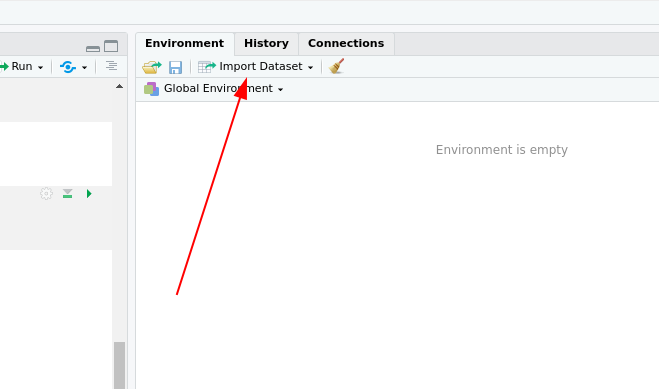
\includegraphics[width=166.666666666667pt]{imgs/menu} \end{center}

\begin{center}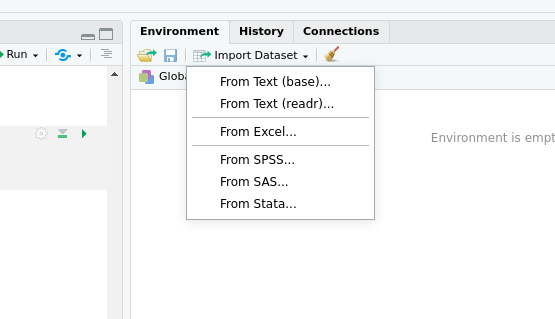
\includegraphics[width=166.666666666667pt]{imgs/menu2} \end{center}

Hier im Beispiel hab ich jetzt die Datei \texttt{test.csv} ausgewählt, die ein Beispiel aus der letzten Vorlesung enthält:

\begin{center}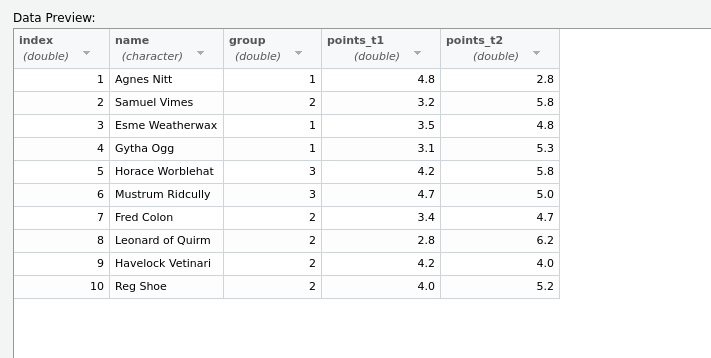
\includegraphics[width=166.666666666667pt]{imgs/text_csv1} \end{center}

Was mir den den folgenden Code-Schnipsel liefert, den ich dann in mein Skript kopieren kann:

\begin{center}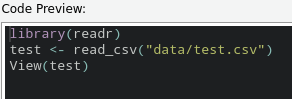
\includegraphics[width=166.666666666667pt]{imgs/text_csv2} \end{center}

\begin{Shaded}
\begin{Highlighting}[]
\NormalTok{test }\OtherTok{\textless{}{-}} \FunctionTok{read\_csv}\NormalTok{(}\StringTok{"data/test.csv"}\NormalTok{)}
\end{Highlighting}
\end{Shaded}

Für's Erste soll uns das an Einlese-Strategien reichen.

\hypertarget{deskriptive-kennwerte}{%
\section{deskriptive Kennwerte}\label{deskriptive-kennwerte}}

\hypertarget{einfache-deskriptiv-statistische-kennwerte-1}{%
\subsection{Einfache deskriptiv-statistische Kennwerte}\label{einfache-deskriptiv-statistische-kennwerte-1}}

Wir hatten in der zweiten Veranstaltung ja schon ein paar deskriptive Kennwerte, die wollen wir jetzt auf Datensätze anwenden.

Wir könnten uns beispielsweise fragen, was der Mittelwert der beiden Punkte pro Testzeitpunkt war.

Dafür können wir die \texttt{pull}-Funktion nutzen, um uns einfache Spalten des Datensatzes als Vektor ausgeben zu lassen:

\begin{Shaded}
\begin{Highlighting}[]
\NormalTok{test }\SpecialCharTok{\%\textgreater{}\%} 
  \FunctionTok{pull}\NormalTok{(points\_t1) }\SpecialCharTok{\%\textgreater{}\%} 
  \FunctionTok{mean}\NormalTok{()}

\NormalTok{test }\SpecialCharTok{\%\textgreater{}\%} 
  \FunctionTok{pull}\NormalTok{(points\_t2) }\SpecialCharTok{\%\textgreater{}\%} 
  \FunctionTok{mean}\NormalTok{()}
\end{Highlighting}
\end{Shaded}

\begin{verbatim}
## [1] 3.79
## [1] 4.96
\end{verbatim}

Das funktioniert zwar, wird aber umständlicher, je mehr Spalten und Kennwerte wir berechnen wollen.

Natürlich gibt es \texttt{tidyverse} auch dafür Funktionen, die uns die Arbeit leichter machen. Mit der \texttt{summarise}-Funktion können wir ähnlich wie mit der \texttt{mutate}-Funktion Variablen definieren, die dann aber Zusammenfassungen über angegebene Funktionen sind:

\begin{Shaded}
\begin{Highlighting}[]
\NormalTok{test }\SpecialCharTok{\%\textgreater{}\%}
  \FunctionTok{summarise}\NormalTok{(}\AttributeTok{m\_t1 =} \FunctionTok{mean}\NormalTok{(points\_t1),}
            \AttributeTok{sd\_t1 =} \FunctionTok{sd}\NormalTok{(points\_t1),}
            \AttributeTok{m\_t2 =} \FunctionTok{mean}\NormalTok{(points\_t2),}
            \AttributeTok{sd\_t2 =} \FunctionTok{sd}\NormalTok{(points\_t2),)}
\end{Highlighting}
\end{Shaded}

\begin{verbatim}
## # A tibble: 1 x 4
##    m_t1 sd_t1  m_t2 sd_t2
##   <dbl> <dbl> <dbl> <dbl>
## 1  3.79 0.689  4.96 0.989
\end{verbatim}

Das ist ja schon ganz nett, aber diese Infos sind selten hilfreich. In unserem Datensatz sind Experimentalgruppen eingeteilt, eigentlich wollen wir unsere Mittelwerte pro Gruppe ausrechnen. Mit der \texttt{group\_by}-Funktion ist das auch ganz einfach möglich.

In unsere \texttt{pipe} von eben bauen wir dazu einfach einen kurzen \texttt{group\_by}-Aufruf ein und schon sind wir beim erwünschten Ergebnis:

\begin{Shaded}
\begin{Highlighting}[]
\NormalTok{test }\SpecialCharTok{\%\textgreater{}\%}
  \FunctionTok{group\_by}\NormalTok{(group) }\SpecialCharTok{\%\textgreater{}\%} 
  \FunctionTok{summarise}\NormalTok{(}\AttributeTok{m\_t1 =} \FunctionTok{mean}\NormalTok{(points\_t1),}
            \AttributeTok{sd\_t1 =} \FunctionTok{sd}\NormalTok{(points\_t1),}
            \AttributeTok{m\_t2 =} \FunctionTok{mean}\NormalTok{(points\_t2),}
            \AttributeTok{sd\_t2 =} \FunctionTok{sd}\NormalTok{(points\_t2))}
\end{Highlighting}
\end{Shaded}

\begin{verbatim}
## # A tibble: 3 x 5
##   group  m_t1 sd_t1  m_t2 sd_t2
##   <dbl> <dbl> <dbl> <dbl> <dbl>
## 1     1  3.8  0.889  4.3  1.32 
## 2     2  3.52 0.576  5.18 0.873
## 3     3  4.45 0.354  5.4  0.566
\end{verbatim}

Und diese Gruppierungen können wir jetzt einfach mit dem vorhin gesehenen \texttt{cut} zur Gruppierung kombinieren.

So könnten wir uns zum Beispiel fragen, wie die Mittelwerte und Streuungen in den Quartilen aussehen. Dafür können wir einfach ein \texttt{mutate} vorschalten, indem wir die Verbesserung zum zweiten Termin und einen Quartilsplit einführen, den wir dann direkt zum Gruppieren benutzen:

\begin{Shaded}
\begin{Highlighting}[]
\NormalTok{test }\OtherTok{\textless{}{-}}\NormalTok{ test }\SpecialCharTok{\%\textgreater{}\%}
  \FunctionTok{mutate}\NormalTok{(}\AttributeTok{improvement =}\NormalTok{ points\_t2 }\SpecialCharTok{{-}}\NormalTok{ points\_t1,}
         \AttributeTok{quart\_split =} \FunctionTok{cut}\NormalTok{(improvement,}
                           \AttributeTok{breaks =} \FunctionTok{c}\NormalTok{(}\SpecialCharTok{{-}}\ConstantTok{Inf}\NormalTok{,}
                                      \FunctionTok{quantile}\NormalTok{(improvement,}
                                               \AttributeTok{probs =} \FunctionTok{c}\NormalTok{(.}\DecValTok{25}\NormalTok{,.}\DecValTok{5}\NormalTok{,.}\DecValTok{75}\NormalTok{)),}
                                      \ConstantTok{Inf}\NormalTok{),}
                           \AttributeTok{right =}\NormalTok{ T,}
                           \AttributeTok{labels =} \FunctionTok{c}\NormalTok{(}\StringTok{\textquotesingle{}q1\textquotesingle{}}\NormalTok{, }\StringTok{\textquotesingle{}q2\textquotesingle{}}\NormalTok{, }\StringTok{\textquotesingle{}q3\textquotesingle{}}\NormalTok{, }\StringTok{\textquotesingle{}q4\textquotesingle{}}\NormalTok{)}
\NormalTok{                           )}
\NormalTok{         ) }

\NormalTok{test }\SpecialCharTok{\%\textgreater{}\%} 
  \FunctionTok{group\_by}\NormalTok{(quart\_split) }\SpecialCharTok{\%\textgreater{}\%} 
  \FunctionTok{summarise}\NormalTok{(}\AttributeTok{m\_t1 =} \FunctionTok{mean}\NormalTok{(points\_t1),}
            \AttributeTok{sd\_t1 =} \FunctionTok{sd}\NormalTok{(points\_t1),}
            \AttributeTok{m\_t2 =} \FunctionTok{mean}\NormalTok{(points\_t2),}
            \AttributeTok{sd\_t2 =} \FunctionTok{sd}\NormalTok{(points\_t2))}
\end{Highlighting}
\end{Shaded}

\begin{verbatim}
## # A tibble: 4 x 5
##   quart_split  m_t1 sd_t1  m_t2 sd_t2
##   <fct>       <dbl> <dbl> <dbl> <dbl>
## 1 q1           4.57 0.321  3.93 1.10 
## 2 q2           3.75 0.354  5    0.283
## 3 q3           3.8  0.566  5.25 0.778
## 4 q4           3.03 0.208  5.77 0.451
\end{verbatim}

\hypertarget{huxe4ufigkeitsauszuxe4hlungen}{%
\subsection{Häufigkeitsauszählungen}\label{huxe4ufigkeitsauszuxe4hlungen}}

Diese \texttt{pipe} können wir auch verwenden, um uns Häufigkeiten von Bedingungskombinationen anzugucken. Dafür tauschen wir einfach die \texttt{summarise}- durch die \texttt{count}-Funktion aus und schon ist der Output eine Tabelle mit den absoluten Häufigkeiten:

\begin{Shaded}
\begin{Highlighting}[]
\NormalTok{test }\SpecialCharTok{\%\textgreater{}\%} 
  \FunctionTok{group\_by}\NormalTok{(quart\_split) }\SpecialCharTok{\%\textgreater{}\%} 
  \FunctionTok{count}\NormalTok{()}
\end{Highlighting}
\end{Shaded}

\begin{verbatim}
## # A tibble: 4 x 2
## # Groups:   quart_split [4]
##   quart_split     n
##   <fct>       <int>
## 1 q1              3
## 2 q2              2
## 3 q3              2
## 4 q4              3
\end{verbatim}

Die \texttt{group\_by}-Funktion kann dabei auch mehrere Argumente verstehen, wir können also auch nach Gruppe und Quantilen auszählen:

\begin{Shaded}
\begin{Highlighting}[]
\NormalTok{test }\SpecialCharTok{\%\textgreater{}\%} 
  \FunctionTok{group\_by}\NormalTok{(quart\_split,group) }\SpecialCharTok{\%\textgreater{}\%} 
  \FunctionTok{count}\NormalTok{()}
\end{Highlighting}
\end{Shaded}

\begin{verbatim}
## # A tibble: 9 x 3
## # Groups:   quart_split, group [9]
##   quart_split group     n
##   <fct>       <dbl> <int>
## 1 q1              1     1
## 2 q1              2     1
## 3 q1              3     1
## 4 q2              1     1
## 5 q2              2     1
## 6 q3              2     1
## 7 q3              3     1
## 8 q4              1     1
## 9 q4              2     2
\end{verbatim}

  \bibliography{book.bib,packages.bib}

\end{document}
